\documentclass[12pt]{article}
\usepackage{esqu1}
\usetikzlibrary{decorations.markings}
\tikzset{
    set arrow inside/.code={\pgfqkeys{/tikz/arrow inside}{#1}},
    set arrow inside={end/.initial=>, opt/.initial=},
    /pgf/decoration/Mark/.style={
        mark/.expanded=at position #1 with
        {
            \noexpand\arrow[\pgfkeysvalueof{/tikz/arrow inside/opt}]{\pgfkeysvalueof{/tikz/arrow inside/end}}
        }
    },
    arrow inside/.style 2 args={
        set arrow inside={#1},
        postaction={
            decorate,decoration={
                markings,Mark/.list={#2}
            }
        }
    },
}
\pagestyle{fancy}

\lhead{Brandon Lin}
\chead{Multivariate Calculus}
\rhead{Fall 2015}


\begin{document}

\title{Multivariate Calculus}
\author{Brandon Lin\\Stuyvesant High School\\Fall 2015\\Teacher: Ms. Avigdor}
\maketitle
\newpage


\tableofcontents
\newpage
\section*{Introduction}
These are the notes from the course I took at Stuyvesant High School, Fall 2015. Note: these are not the exact notes that were taken; these notes skip some properties that should be obvious if you took precalculus.
\section{3 Dimensional Space}
A \textbf{plane} can be represented by the equation $Ax + By + Cz + D = 0$. 
\begin{itemize}
\item When one of $A,B,C$ is nonzero, the plane is parallel to a \textbf{coordinate plane} (the $xy$-plane, $xz$-plane, or $yz$-plane).
\item When two of them are nonzero, the plane is paralle to a coordinate axis.
\item When all of them are nonzero, the plane intersects all three axes.
\end{itemize}

A \textbf{cylinder} is a surface that consists of all lines parallel to a given line and passing through a given curve. 

For example, a \textbf{right circular cylinder} can be represented by the equation $x^2 + (z-3)^2 = 4$. This cylinder has an axis of symmetry parallel to the $y$-axis, and has radius 2.

To graph an arbitrary surface/cylinder, we look at the \textbf{traces} that the surface makes with the coordinates planes and any planes parallel to the coordinate axes. The traces are the intersection between the two. For example, if we wish to look at the traces that the cylinder makes with the $xy$-plane, we let $z=0$ (the equation for the $xy$-plane) and see what equation that gives us on the plane. Likewise, to get the trace for any plane parallel to that $xy$-plane, we let $z=k$, and we find the intersection of the surface and the plane keeping $k$ constant.

\section{Vectors}
\subsection{Properties of Vectors}
\begin{itemize}
\item $\vec{u} + \vec{v} = \vec{v} + \vec{u}$ (Commutative)
\item $(\vec{u} + \vec{v}) + \vec{w} = \vec{u} + (\vec{v} + \vec{w})$ (Associative)
\item $\vec{u} + \vec{0} = \vec{0} + \vec{u} = \vec{u}$ (Identity Element under addition)
\item $\vec{u} + (-\vec{u}) = \vec{0}$ (Additive Inverse)
\item $c(\vec{u} + \vec{v}) = c\vec{u} + c\vec{v}$ (Distributive, vector)
\item $(c+d)\vec{u} = c\vec{u} + d\vec{u}$ (Distributive, scalar)
\item $c(d\vec{u}) = (cd)\vec{u}$ (Mixed Associative)
\item $1\vec{u} = \vec{u}$ (Identity Element)
\end{itemize}

\subsection{The Dot/Scalar Product}
If $\vec{u} = \la u_1, u_2, \dots, u_n \ra$ and $\vec{v} = \la v_1, v_2, \dots, v_n \ra$, then \[ \vec{u} \cdot \vec{v} = u_1v_1 + u_2v_2 + \cdots + u_nv_n = \sum_{i = 1}^n{u_iv_i} \]
\begin{figure}[h!]
\centering
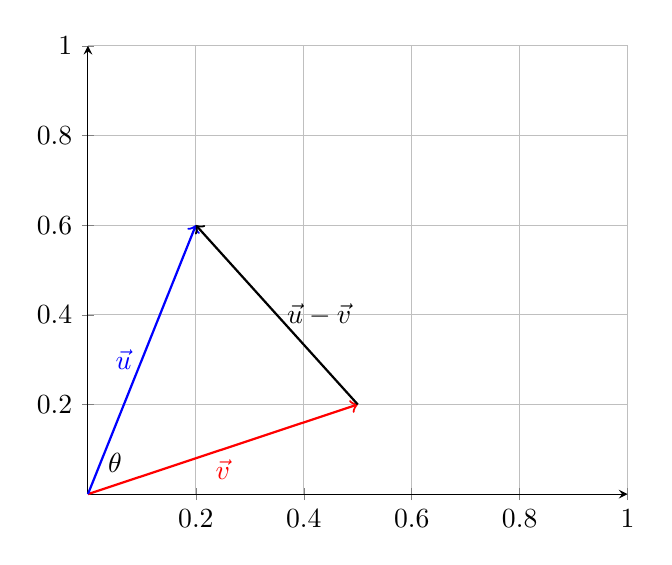
\begin{tikzpicture}
\begin{axis}[grid=major,axis x line=middle,
             axis y line=middle,
             after end axis/.code={
               \draw[red,thick,->] (axis cs:0,0) -- (axis cs:0.5,0.2) node[midway,below]{$\vec{v}$};
               \draw[blue,thick,->] (axis cs:0,0) -- (axis cs:0.2,0.6) node[midway,left]{$\vec{u}$}; 
               \draw[black,thick,->] (axis cs:0.5,0.2) -- (axis cs:0.2,0.6) node[midway,right]{$\vec{u} - \vec{v}$};
               \node at (axis cs:0.05,0.07){$\theta$};
  }]
\end{axis}
\end{tikzpicture}
\end{figure}
Let $\theta$ denote the angle between $\vec{u}$ and $\vec{v}$. Using the Law of Cosines, 
\[
\begin{aligned}
\norm{\vec{u} - \vec{v}}^2 &= (\vec{u} - \vec{v})\cdot(\vec{u} - \vec{v}) = \norm{\vec{u}}^2 + \norm{\vec{v}}^2 - 2\norm{\vec{u}}\norm{\vec{v}}\cos{\theta} \\
\norm{\vec{u}}^2 - 2(\vec{u}\cdot\vec{v}) + \norm{\vec{v}}^2 &= \norm{\vec{u}}^2 + \norm{\vec{v}}^2 - 2\norm{\vec{u}}\norm{\vec{v}}\cos{\theta} \\ 
&\to \boxed{\vec{u}\cdot\vec{v} = \norm{\vec{u}}\norm{\vec{v}}\cos{\theta}} \\
\end{aligned}
\]
This is the geometric definition of the dot product, which allows us to find the angle between two vectors easily.

\subsection{The Cauchy-Schwarz Inequality, Triangle Inequality}
\begin{theorem}[Cauchy-Schwarz Inequality]
If $\vec{u}$ and $\vec{v}$ are vectors in $\mathbb{R}^n$, then $|\vec{u}\cdot\vec{v}| \le \norm{\vec{u}}\norm{\vec{v}}$.
\end{theorem}

\begin{proof}
Rearranging the geometric definition of the dot product, we get $\cos{\theta} = \frac{\vec{u} \cdot \vec{v}}{\norm{\vec{u}}\norm{\vec{v}}}$. And since $|\cos{\theta}| \le 1$, we get that $ \left|\frac{\vec{u} \cdot \vec{v}}{\norm{\vec{u}}\norm{\vec{v}}}\right| \le 1 \to |\vec{u} \cdot \vec{v}| \le \norm{\vec{u}}\norm{\vec{v}}$.
\end{proof}

\begin{theorem}[Triangle Inequality]
If $\vec{u}$ and $\vec{v}$ are vectors in $\mathbb{R}^n$, then $\norm{\vec{u} + \vec{v}} \le \norm{\vec{u}} + \norm{\vec{v}}$.
\end{theorem}

\begin{proof}
\[
\begin{aligned}
\norm{\vec{u} + \vec{v}}^2 &= (\vec{u} + \vec{v})\cdot(\vec{u} + \vec{v}) \\
&= \vec{u}\cdot\vec{u} + 2(\vec{u}\cdot\vec{v}) + \vec{v}\cdot\vec{v} \\
&\le \norm{\vec{u}}^2 + 2|\vec{u}\cdot\vec{v}| + \norm{\vec{v}}^2  \\
\end{aligned}
\]
By Cauchy-Schwarz:
\[
\begin{aligned}
\norm{\vec{u} + \vec{v}}^2 &\le \norm{\vec{u}}^2 + 2\norm{\vec{u}}\norm{\vec{v}} + \norm{\vec{v}}^2 \\
&= (\norm{\vec{u}} + \norm{\vec{v}})^2 \\
\norm{\vec{u} + \vec{v}} &\le \norm{\vec{u}} + \norm{\vec{v}}
\end{aligned}
\]
\end{proof}

\subsection{Projections}
\begin{figure}[h!]
\centering
\begin{tikzpicture}
\coordinate (a) at (10,0);
\coordinate (b) at (2.5,3);
\coordinate (o) at (0,0);
\coordinate (c) at (2.5,0);
\draw[red,thick,->] (o) -- (a) node[midway,below]{$\vec{a}$};
\draw[blue,thick,->] (o) -- (b) node[midway,above]{$\vec{b}$};
\draw[green,->] (o) -- (c) node[midway,below]{$\proj_{\vec{a}}{\vec{b}}$};
\draw[dotted] (b) -- (c);
\node at (10.2,0) {$A$};
\node at (-0.2,-0.2) {$O$};
\node at (2.5,-0.2) {$C$};
\node at (2.7,3.2) {$B$};
\node at (0.5,0.2) {$\alpha$};
\end{tikzpicture}
\end{figure}
$\overrightarrow{OC}$ is the vector projection  of $\overrightarrow{OB}$ ($\vec{b}$) onto $\overrightarrow{OA}$ ($\vec{a}$). This is denoted as $\proj_{\vec{a}}{\vec{b}}$. \\
The magnitude of this projection, $\norm{\overrightarrow{OC}}$, is denoted as $\comp_{\vec{a}}{\vec{b}}$. \\ \\
To describe $\overrightarrow{OC}$, we need its direction and magnitude.
\begin{itemize}
\item Direction is given by the unit vector in the direction if $\vec{a}$, which is $\frac{\vec{a}}{\norm{\vec{a}}}$.
\item Magnitude is given by:
\[
\begin{aligned}
\norm{\overrightarrow{OC}} &= \norm{\vec{b}}\cos{\alpha} \\
&= \norm{\vec{b}} \frac{\vec{a} \cdot \vec{b}}{\norm{\vec{a}}\norm{\vec{b}}} = \frac{\vec{a} \cdot \vec{b}}{\norm{\vec{a}}}
\end{aligned}
\]
Therefore, \[ 
\begin{aligned}
\overrightarrow{OC} &= \frac{\vec{a} \cdot \vec{b}}{\norm{\vec{a}}}\left(\frac{\vec{a}}{\norm{\vec{a}}}\right) = \frac{\vec{a} \cdot \vec{b}}{\norm{\vec{a}}^2} \\ 
\Aboxed{\proj_{\vec{a}}{\vec{b}} &= \frac{\vec{a} \cdot \vec{b}}{\norm{\vec{a}}^2}\vec{a}}
\end{aligned}
\]
\end{itemize}

We can also easily see that, from this,  $\boxed{\comp_{\vec{a}}{\vec{b}} = \dfrac{\vec{a} \cdot \vec{b}}{\norm{\vec{a}}}}$.

\subsection{Direction Cosines}
In 3-space, the direction cosines give the cosines of the angles formed between a vector and the three axes.

If $\alpha, \beta, \gamma$ are the angles that the vector $\vec{A} = \la A_x, A_y, A_z \ra$ makes with the $x$, $y$, and $z$ axes respectively, then:
\[
\begin{aligned}
\vec{A} &= \la A_x, A_y, A_z \ra \\
&= \la \norm{\vec{A}}\cos{\alpha}, \norm{\vec{A}}\cos{\beta}, \norm{\vec{A}}\cos{\gamma} \\
&= \norm{\vec{A}} \la \cos{\alpha}, \cos{\beta}, \cos{\gamma} \ra
\end{aligned}
\]

\subsection{The Cross/Vector Product}
The cross product returns a vector that is orthogonal (perpendicular) to the two vectors in question. 

The proof is omitted, but if $\vec{a}$ and $\vec{b}$ are vectors, then 
\[ \vec{a} \times \vec{b} =
\begin{vmatrix}
\ihat & \jhat & \khat \\
a_1 & a_2 & a_3 \\
b_1 & b_2 & b_3 
\end{vmatrix} 
\]

The magnitude of this vector is given by: \[ \norm{\vec{a} \times \vec{b}} = \norm{\vec{a}}\norm{\vec{b}}\sin{\theta} \]

The direction of this vector is orthogonal to the vector, but which direction exactly? We have two different options. The convention is to use the right-hand rule: point your fingers towards $\vec{a}$ and sweep them towards your palm towards $\vec{b}$. Your thumb points in the direction of the product.

\subsection{Volume of a Parallelogram}
\begin{figure}[h!]
\centering
\begin{tikzpicture}
\coordinate (a) at (10,0);
\coordinate (b) at (2.5,3);
\coordinate (o) at (0,0);
\coordinate (c) at (2.5,0);
\coordinate (d) at (12.5,3);
\draw[red,thick,->] (o) -- (a) node[midway,below]{$\vec{a}$};
\draw[blue,thick,->] (o) -- (b) node[midway,above]{$\vec{b}$};
\draw[black] (a) -- (d) -- (b);
\draw[dotted] (b) -- (c) node[midway,left]{$h$};
\node at (10.2,0) {$A$};
\node at (-0.2,-0.2) {$O$};
\node at (2.5,-0.2) {$C$};
\node at (2.7,3.2) {$B$};
\node at (0.5,0.2) {$\alpha$};
\end{tikzpicture}
\end{figure}


\[
\begin{aligned}
\text{Area} &= bh \\
b &= \norm{\vec{a}}, h = \norm{\vec{b}}\sin{\alpha} \\
\text{Area} &= \norm{\vec{a}}\norm{\vec{b}}\sin{\alpha} \\
\Aboxed{\text{Area} &= \norm{\vec{a} \times \vec{b}}}
\end{aligned}
\]
\newpage
\subsection{Volume of a Parallelepiped}

\begin{figure}[h!]
\centering
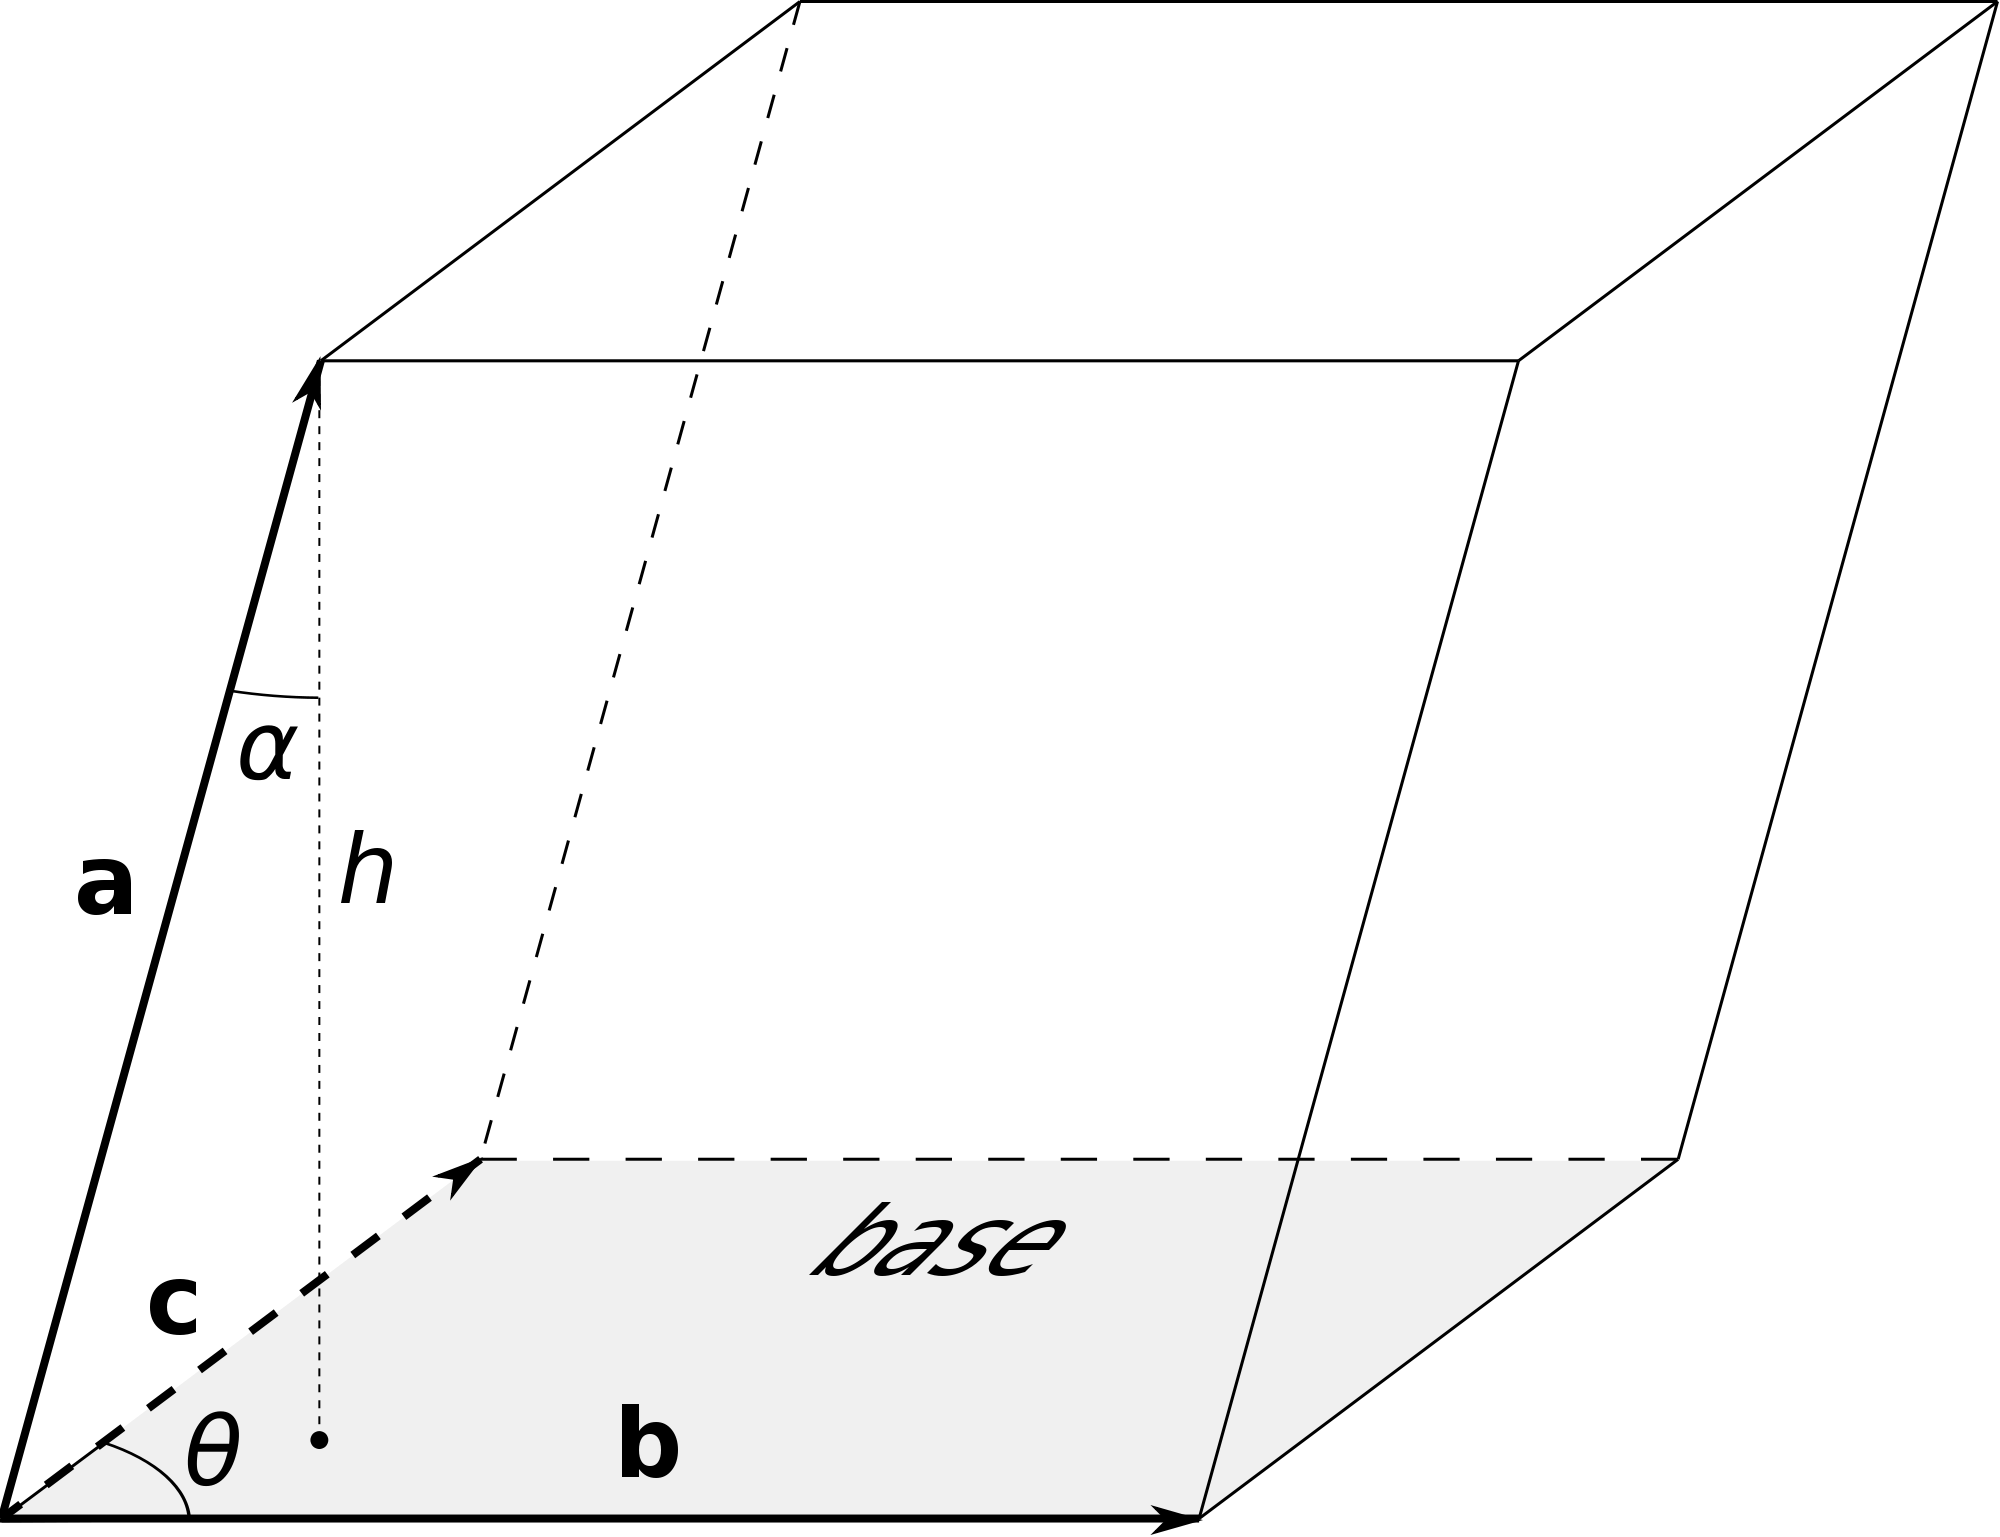
\includegraphics[scale=0.1]{box}
\end{figure}

\[
\begin{aligned}
\text{Volume} &= Bh \\ 
\Aboxed{\text{Volume} &= (\vec{b} \times \vec{c}) \cdot \vec{a}}
\end{aligned}
\]

\section{Lines and Planes in Space}
\subsection{Lines}
To find an equation for a line, we need a specific point on the plane, as well as a vector that points in the direction of the line. Representing the specific point as a vector, Let $\vec{r_0} = \la x_0,y_0,z_0 \ra$ be the initial vector and $\vec{v} = \la a,b,c \ra$ be the vector that points in the direction of the line.

Then, we can hit all such points on the line and represent any arbitrary point as $\vec{r_0} + t\vec{v}$, where $t$ is a parameter. As $t$ varies, we will hit all the points on the line. This gives rise to three forms of the equation of a line:
\begin{itemize}
\item Vector form:
\[ \vec{r} = \vec{r_0} + t\vec{v} \]
\item Parametric form:
\[
\begin{cases}
x = x_0 + at \\
y = y_0 + bt \\ 
z = z_0 + ct
\end{cases}
\]
\item Symmetric form\footnote{This can be derived by isolating $t$ in the above equations and setting them equal to each other.}:
\[ \frac{x - x_0}{a} = \frac{y - y_0}{b} = \frac{z - z_0}{c} \]
\end{itemize}

\subsection{Planes}
Let $P_0(x_0,y_0,z_0)$ be a given point on a plane, and $P(x,y,z)$ an arbitrary point on the plane. Let $\vec{n}$ be the normal\footnote{Orthogonal/perpendicular.} to the plane at $P_0$. Now since $\vec{n} \perp \overrightarrow{P_0P}$, we have that
\[
\begin{aligned}
\vec{n} \cdot \overrightarrow{P_0P} &= 0 \\ 
\la a,b,c \ra \cdot \la x-x_0, y-y_0, z-z_0 \ra &= 0 \\
\Aboxed{a(x-x_0) + b(y-y_0) + c(z-z_0) &= 0} 
\end{aligned}
\]

This is the \textbf{point-normal form} of the equation of the line. We could also move the constant terms to one side to obtain $ax+by+cz = d$, the \textbf{standard form} of the equation.

\section{Vector-Valued Functions}
\subsection{Definitions}
A vector valued function $\vec{r}(t)$ is a function that takes in a scalar and returns a vector. We denote the function as such:
\[
\begin{aligned}
\vec{r}(t) &= f(t)\ihat + g(t)\jhat + h(t)\khat \\
&= \la f(t), g(t), h(t) \ra
\end{aligned}
\]
where $f(t), g(t), h(t)$ are scalar-valued functions. We can assess the domain of $\vec{r}(t)$ by looking at the domain of the individual scalar valued functions. We can also define a limit\footnote{This limit is both additive and multiplicative with dot/cross products.} as follows:
\[ \lim_{t\rightarrow a}{\vec{r}(t)} = \left\la \lim_{t\rightarrow a}{f(t)}, \lim_{t\rightarrow a}{g(t)}, \lim_{t\rightarrow a}{h(t)} \right\ra \]
\subsection{Continuity}
$\vec{r}(t)$ is continuous at $t=a$ IFF:
\begin{enumerate}
\item $\displaystyle\lim_{t\rightarrow a}{\vec{r}(t)}$ exists
\item $\vec{r}(a)$ exists
\item $\displaystyle\lim_{t\rightarrow a}{\vec{r}(t)} = \vec{r}(a)$
\end{enumerate}

\subsection{Derivatives}
We can also define the derivative of a vector-valued function as $\pvec{r}'(t)$. The proof for finding the derivative of a vector-valued function is analagous to that of a scalar-valued function, just repeated multiple times, so it will be omitted here.
\[ \pvec{r}'(t) = f'(t)\ihat + g'(t)\jhat + h'(t)\khat \]

\subsection{Unit Tangent/Normal Vectors}
We define a \textbf{smooth} curve/function as one that is continuous everywhere and where $\pvec{r}'(t) \neq 0$. \\ \\
Here, we need two special vectors associated with tangent vectors. We can define the \textbf{unit tangent vector} as follows:
\[ \vec{T}(t) = \frac{\pvec{r}'(t)}{\norm{\pvec{r}'(t)}}\]

Now, suppose that $\vec{r}(t)$ is twice differentiable. Since $\vec{T}(t)$ is a unit vector,
\[
\begin{aligned}
\vec{T}(t) \cdot \vec{T}(t) &= 1 \\
\frac{d}{dt}(\vec{T}(t) \cdot \vec{T}(t)) &= \frac{d}{dt}(1) \\
2{[}\pvec{T}'(t) \cdot \vec{T}(t) {]} &= 0 \\
\pvec{T}'(t) \cdot \vec{T}(t) &= 0 \\
\end{aligned}
\]
which means $\pvec{T}'(t)$ is orthogonal to $\vec{T}(t)$. We can define a unit vector in the direction of $\pvec{T}'(t)$, known as the \textbf{unit normal vector}:
\[ \vec{N}(t) = \frac{\pvec{T}'(t)}{\norm{\pvec{T}'(t)}} \]

\subsection{Arc Length}
The arc length along a curve $\vec{r}(t)$ from starting point $t=a$ is:
\[ s(t) = \int_a^t{\norm{\pvec{r}'(t)} \ dt} \]

We can parameterize a curve with arc length, meaning the input will be the length traveled along a curve and the function will return the position. 

To do so, we first find the arc length function in terms of $t$. Then, we get $t$ in terms of the arc length, and substitute this expression into the curve's function. 

We prove two results of this:

\begin{theorem}
This technique does yield an arc length parameterization.
\end{theorem}

\begin{proof}
Let $\vec{r}(t)$ be a parameterization of the curve.
\[ s(t) = \int_a^t\norm{\pvec{r}'(u)} \ du \rightarrow s'(t) = \norm{\pvec{r}'(t)} > 0 \]
which means $s(t)$ willl always have an inverse. Call this inverse $\varphi(s) = t$. \\ \\
Let $\vec{r_1}(s) = \vec{r}(\varphi(s))$; this is our new parameterization. We wish to show that $\norm{\pvec{r_1}'(s)} = 1$.\footnote{If this is the case, then the formula for arc length yields the proper arc length.} 

\[
\begin{aligned}
\norm{\pvec{r_1}'(s)} &= \norm{\frac{d}{ds}{[}\vec{r}(\phi(s)){]}} \\
&= \norm{\varphi'(s)\pvec{r}'(\varphi(s))} \\
&= \norm{\varphi'(s)}\norm{\pvec{r}'(\varphi(s))}
\end{aligned}
\]
Do note that $\pvec{r}'(\phi(s))$ is $\pvec{r}'(t)$ EVALUATED at $t = \varphi(s)$. Then,
\[
\begin{aligned}
\varphi'(s) = \dfrac{dt}{ds} &= \frac{1}{\frac{ds}{dt}} \\
&= \frac{1}{s'(t)} \\
&= \frac{1}{s'(\varphi(s))} \\
&= \frac{1}{\norm{\pvec{r}'(\varphi(s))}}
\end{aligned}
\]
Substituting:
\[ \norm{\pvec{r_1}'(s)} = \norm{\varphi'(s)}\norm{\pvec{r}'(\varphi(s))} = \frac{1}{\norm{\pvec{r}'(\varphi(s))}} \norm{\pvec{r}'(\varphi(s))} = 1 \]
\end{proof}

\begin{theorem}
The arc length is invariant under different parameterizations.
\end{theorem}

\begin{proof}
Let $\vec{r}(t)$ and $\vec{R}(u)$ be two different parameterizations of the same curve. We will run the arc length along $a \le t \le b$ and $c \le u \le d$, so we relate the two paramters $t$ and $u$ with the equation $t = \phi(u)$. Note that $\vec{r}(\phi(u) = R(u)$. \\ \\
We need to show that $\int_a^b\norm{\pvec{r}'(t)} \ dt = \int_c^d\norm{\pvec{R}'(u)} \ du$.

Noting that $dt = \phi'(u) \ du$, we do u-substitution:
\[
\begin{aligned}
\int_a^b\norm{\pvec{r}'(t)} \ dt &= \int_c^d\norm{\pvec{r}'(\phi(u))} \phi'(u) \ du \\
&= \int_c^d\norm{\phi'(u)\pvec{r}'(\phi(u))} \ du \\
&= \int_c^d\norm{\frac{d}{du}\vec{r}(\phi(u))} \ du \\
&= \int_c^d\norm{\pvec{R}'(u)} \ du
\end{aligned}
\]
\end{proof}
\newpage
\subsection{Curvature}
\textbf{Curvature}, represented by the Greek letter $\kappa$ (kappa), is how fast the direction of a certain curve is changing. We will look at two definitions of curvature. We prove the result for plane curves, but the results can be extended to space curves.
\begin{enumerate}
\item $\kappa = \left|\frac{d\theta}{ds}\right|$ \\
\begin{figure}[h!]
\centering
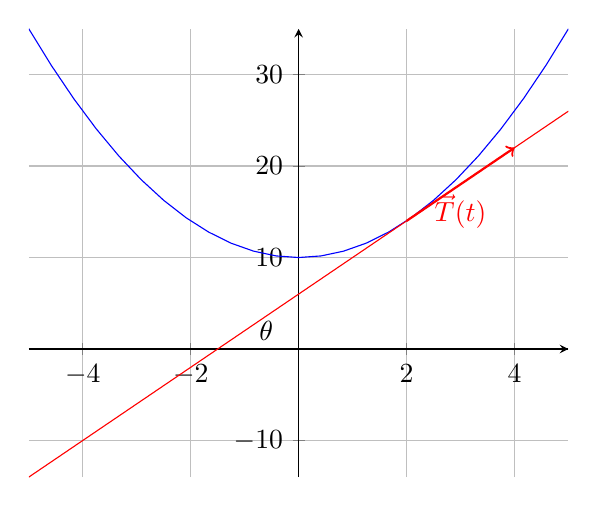
\begin{tikzpicture}
\begin{axis}[grid=major,axis x line=middle,
             axis y line=middle,
             after end axis/.code={
               \draw[red,thick,->] (axis cs:2,14) -- (axis cs:4,22) node[midway,below]{$\vec{T}(t)$};
               \node at (axis cs:-0.6,2) {$\theta$};
  }]

\addplot[color=blue]{x^2+10};
\addplot[color=black]{0};
\addplot[color=red]{4*x+6};
\end{axis}
\end{tikzpicture}
\end{figure}
Suppose $\vec{r}(t) = \la x(t), y(t) \ra$. Note that \[ \tan{\theta} = \frac{dy}{dx} = \dfrac{\frac{dy}{dt}}{\frac{dx}{dt}} = \frac{y'(t)}{x'(t)} \]
And $\theta = \tan^{-1}\left(\frac{y'(t)}{x'(t)}\right)$. Since $\frac{d\theta}{ds} = \frac{d\theta}{dt}\frac{dt}{ds}$ by the Chain Rule, then,
\[ 
\begin{aligned}
\frac{d\theta}{dt} &= \dfrac{1}{1 + {[}\frac{y'(t)}{x'(t)}{]}^2} \cdot \frac{d}{dt}\left(\frac{y'(t)}{x'(t)}\right) \\
\frac{dt}{ds} &= \dfrac{1}{\frac{ds}{dt}} = \frac{1}{\sqrt{{[}x'(t){]}^2 + {[}y'(t){]}^2}} \\
\frac{d\theta}{ds} &= \dfrac{1}{1 + {[}\frac{y'(t)}{x'(t)}{]}^2} \cdot \frac{d}{dt}\left(\frac{y'(t)}{x'(t)}\right) \cdot  \frac{1}{\sqrt{{[}x'(t){]}^2 + {[}y'(t){]}^2}} \\
&= \dfrac{x'y''-y'x''}{{[}(x')^2+(y')^2{]}^{\frac{3}{2}}} \\
\Aboxed{\kappa &= \dfrac{\norm{\pvec{r}'(t) \times \pvec{r}''(t)}}{\norm{\pvec{r}'(t)}^3}} \\
\end{aligned}
\]
\item $\kappa = \norm{\frac{d\vec{T}}{ds}}$
\[ 
\begin{aligned}
\frac{d\vec{T}}{ds} &= \frac{d\vec{T}}{dt} \frac{dt}{ds} = \frac{\pvec{T}'(t)}{\norm{\pvec{r}'(t)}} \\
\left|\left|\frac{d\vec{T}}{ds}\right|\right| &= \boxed{\kappa = \frac{\norm{\pvec{T}'(t)}}{\norm{\pvec{r}'(t)}}}
\end{aligned}
\]
\end{enumerate}

Now we show these two expressions are equivalent, namely the following theorem:

\begin{theorem}
The curvature of a curve $\vec{r}(t)$ is given by $\kappa = \left|\left|\frac{d\vec{T}}{ds}\right|\right| = \dfrac{\norm{\pvec{r}'(t) \times \pvec{r}''(t)}}{\norm{\pvec{r}'(t)}^3}$
\end{theorem}

\begin{proof}
By definition, $\vec{T}(t) = \frac{\pvec{r}'(t)}{\norm{\pvec{r}'(t)}}$ and $\norm{\pvec{r}'(t)} = s'(t)$, so we can write \[ \pvec{r}'(t) = s'(t)\pvec{T}'(t) \]
Differentiating, we get \[ \pvec{r}''(t) = s''(t)\pvec{T}(t) + s'(t)\pvec{T}'(t) \]
Then,
\[
\begin{aligned}
\pvec{r}'(t) \times \pvec{r}''(t) &= s'(t)\pvec{T}(t) \times {[}s''(t)\pvec{T}(t) + s'(t)\pvec{T}'(t){]} \\ 
&= {[}s'(t)\pvec{T}(t) \times s''(t)\pvec{T}(t){]} + {[}s'(t)\pvec{T}(t) \times s'(t)\pvec{T}'(t){]} \\
&= \underbrace{s'(t)s''(t){[}\pvec{T}(t) \times \pvec{T}(t){]}}_{\vec{0}} + {[}s'(t){]}^2{[}\pvec{T}(t) \times \pvec{T}'(t){]} \\
&= {[}s'(t){]}^2{[}\pvec{T}(t) \times \pvec{T}'(t){]} \\ \\
\norm{\pvec{T}(t) \times \pvec{T}'(t)} &= \norm{\pvec{T}(t)}\norm{\pvec{T}'(t)}\sin{\frac{\pi}{2}} \\
&= \norm{\pvec{T}'(t)} \\ \\
\norm{\pvec{r}(t) \times \pvec{r}'(t)} &= {[}s'(t){]}^2\norm{\pvec{T}'(t)} \\
&= \norm{\pvec{r}'(t)}^2\norm{\pvec{T}'(t)} \\
&= \norm{\pvec{r}'(t)}^2(\norm{\pvec{r}'(t)}\kappa) \\
\kappa &= \dfrac{\norm{\pvec{r}'(t) \times \pvec{r}''(t)}}{\norm{\pvec{r}'(t)}^3}
\end{aligned}
\]
\end{proof}

By considering the curve $\vec{r}(t) = \la a\cos{t}, a\sin{t}, 0 \ra$, which is the path of a circle, you can prove that the curvature of a circle with radius $a$ is $\kappa = \frac{1}{a}$.

It is also possible to prove (the details are not shown here) that for a function $y = f(x)$, the curvature is given by:
\[ \kappa(x) = \dfrac{|f''(x)|}{{[}1+{[}f'(x){]}^2{]}^{\frac{3}{2}}} \]

\subsection{The Osculating Circle}
An \textbf{osculating circle} at a point $P$ on a curve $C$:
\begin{itemize}
\item Has the same curvature as $C$ at $P$
\item Same tangent vector/tangent line
\item Same principal normal vector
\item Has radius $\frac{1}{\kappa}$
\end{itemize}

\subsection{Binormal Vector}
The \textbf{binormal vector}, defined as $\vec{B} = \vec{T} \times \vec{N}$, enables us to create a moving coordinate system of a particle moving along a curve. We can define the coordinate planes of this reference frame:
\begin{itemize}
\item The \textbf{osculating plane}, consisting of $\vec{T}$ and $\vec{N}$
\item The \textbf{normal plane}, consisting of $\vec{N}$ and $\vec{B}$
\item The \textbf{rectifying plane}, consisting of $\vec{T}$ and $\vec{B}$
\end{itemize}

\subsection{Motion in Space}
Using basic knowledge of physics, the velocity vector of a particle following the path $\vec{r}(t)$ is given by $\vec{v}(t) = \pvec{r}'(t)$, and the acceleration is given by $\vec{a}(t) = \pvec{r}''(t)$. We can also get the speed as the magnitude of the velocity, which is $v(t) = \norm{\pvec{r}'(t)}$.

However, it is useful to know what the tangential and normal components of acceleration are rather than solely the $x$ and $y$ components. Here, we derive the formulas for those.

Recall that \[ \pvec{T}(t) = \frac{\pvec{r}'(t)}{\norm{\pvec{r}'(t)}} = \frac{v(t)}{\norm{\vec{v}(t)}} \rightarrow \vec{v}(t) = v(t)\vec{T}(t) \]

Differentiating: \[ \vec{a}(t) = v'(t)\vec{T}(t) + v(t)\pvec{T}'(t) \]

Recall that $\pvec{N}(t) = \frac{\pvec{T}'(t)}{\norm{\pvec{T}'(t)}} \rightarrow \pvec{T}'(t) = \norm{\pvec{T}'(t)}\vec{N}(t)$, and that $\kappa = \frac{\norm{\pvec{T}'(t)}}{\norm{\pvec{r}'(t)}} \rightarrow \norm{\pvec{T}'(t)} = \kappa v(t)$ 

Substituting: \[ \vec{a}(t) = v'(t)\vec{T}(t) + \kappa{[}v(t){]}^2\vec{N}(t) \]

The tangential component is given by $a_T = v'(t)$, and the normal component is given by $a_N = \kappa{[}v(t){]}^2$. 

There are other formulas for these:
\[
\begin{aligned}
a_T &= \frac{\pvec{r}'(t) \cdot \pvec{r}''(t)}{\norm{\pvec{r}'(t)}} \\
a_N &= \frac{\norm{\pvec{r}'(t) \times \pvec{r}''(t)}}{\norm{\pvec{r}'(t)}}
\end{aligned}
\]

I don't have the proofs of these on me now; they're on a handout somewhere that I'm trying to find.

\section{Multivariate Functions}
A function of $n$-variables $x_1,x_2,\dots,x_n$ is a rule that maps/assigns to each $n$-tuple in a set $D \subseteq \mathbb{R}^n$ a unique value $z = f(x_1,x_2,\dots,x_n) \in \mathbb{R}$. In other words, $f:\mathbb{R}^n \rightarrow \mathbb{R}$.

We introduce some terminology to discuss sets in Euclidean space:
\begin{itemize}
\item $(x_0,y_0)$ is an \textbf{interior point} of a region $\mathcal{R}$ if it is the center of a disk contained entirely within $\mathcal{R}$.
\item $(x_0,y_0)$ is a \textbf{boundary point} of a region $\mathcal{R}$ if all such disks centered at $(x_0,y_0)$ contain both exterior and interior points.
\item An \textbf{open region} consists solely of interior points.
\item A \textbf{closed region} consists of both interior and boundary points.
\item A \textbf{bounded region} can be contained within a disk of finite radius.
\item An \textbf{unbounded region} cannot be contained within a disk of finite radius.
\end{itemize}

\subsection{Function Notation}
There are 2 forms:
\begin{itemize}
\item Explicit form: $z = f(x_1,x_2,\dots,x_n)$
\item Implicit form: $F(x_1,x_2,\dots,x_n,z) = 0$
\end{itemize}

The graph of a multivariate function of 2 variables $z=f(x,y)$ is called a \textbf{surface} and consists of all points $(x,y,z)$ for which $z = f(x,y)$ and $(x,y)$ is in the domain of $f$. We can extend this to functions of 3-variables; however, we can't physically draw the graph as it would involve 4-dimensional space$\dots$

\subsection{Level Curves}
A \textbf{level curve} is the set of all points $(x,y)$ in the domain of $f$  such that $f(x,y) = k$. If we envision the surface on a graph, the level curves would give all the points at the same elevation from the $xy$-plane. By combining multiple level curves, we can create a contour map of a function's graph.

Note that two level curves will never intersect; if they intersected, say at a point $(x_0,y_0)$, then $f(x_0,y_0)$ would take on two different values, a contradiction.

\begin{figure}[h!]
\centering
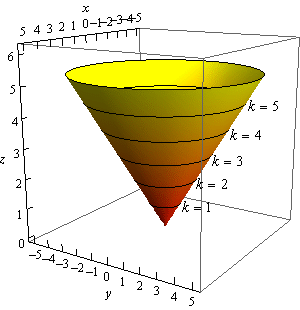
\includegraphics[scale=0.5]{level}
\end{figure}

\subsection{Limits of Multivariate Functions}
Previously when we defined limits for single-variable functions, $x$ would approach a certain value $a$ along the $x$-axis either from the positive direction or the negative direction, so we could check both to make sure that they exist and are equal. However, in a multivariate function, there are infinitely many ways to approach a point $(x_0,y_0)$, via different paths. Therefore, we cannot take limits as easily as before; there is no special L'Hopital's Rule for this. \\ \\
For example, consider:
\[ \lim_{(x,y) \rightarrow (0,0)}{\frac{-3xy}{x^2+y^2}} \]
If we try and plug in $(0,0)$ directly, we get $\frac{0}{0}$, which is not possible. So instead, we choose a path that we can take the limit on.

We can first let $y=0$; then the limit becomes \[ \lim_{(x,0) \rightarrow (0,0)}{\frac{-3x(0)}{x^2+(0)^2}} = \lim_{(x,0) \rightarrow (0,0)}{0} = 0 \]
However, if we let $y = x$: \[ \lim_{(x,x) \rightarrow (0,0)}{\frac{-3x^2}{2x^2}} = \lim_{(x,x) \rightarrow (0,0)}{-\frac{3}{2}} = \frac{3}{2} \]
But we have obtained two different values for the limit. Therefore, this limit does not exist.

One other way you can compute limits in two dimensions is to use polar coordinates. Note that as $(x,y) \rightarrow (0,0)$, then $r \rightarrow 0$, so we can convert our initial problem into a single variable limit. In our example:

\[ 
\begin{aligned}
\lim_{(x,y) \rightarrow (0,0)}{\frac{-3xy}{x^2+y^2}} &= \lim_{r \rightarrow 0}{\frac{-3(r\cos{\theta})(r\sin{\theta})}{(r\cos{\theta})^2 + (r\sin{\theta})^2}} \\
&= \lim_{r \rightarrow 0}{\frac{-3r^2\cos{\theta}\sin{\theta}}{r^2(\cos^2{\theta} + \sin^2{\theta})}} \\
&= \lim_{r \rightarrow 0}{-\frac{3}{2}\sin{2\theta}} 
\end{aligned}
\]

But this limit does not exist, since we know nothing about the value of $\theta$ or where it's approaching.

\subsection{Partial Derivatives}
Now, we investigate rates of changes in multivariate functions. In a function of two variables $z = f(x,y)$, it is often useful to see how the function behaves in the $x$ and the $y$ directions. This can be accomplished by holding one of the variables constant, and allowing the other one to vary. 

If we hold $y$ constant, say at $y = y_0$, then $z = f(x,y_0)$ is now a function of one variable, and we can analyze the rate of change with respect to $x$ by taking $\frac{d}{dx}$. In multivariate functions, these are known as \textbf{partial derivatives}, denoted and defined as:
\[
\begin{aligned}
\frac{\partial f}{\partial x} &= f_x(x,y) = \lim_{\Delta x \rightarrow 0}{\frac{f(x+\Delta x,y) - f(x,y)}{\Delta x}} \\
\frac{\partial f}{\partial y} &= f_y(x,y) = \lim_{\Delta y \rightarrow 0}{\frac{f(x,y+\Delta y) - f(x,y)}{\Delta y}}
\end{aligned}
\]

Note that the partial derivative (in this case, w.r.t. $x$) actually give us the slope of the tangent line at $(a,b)$ to the curve of intersection of the surface $z = f(x,y)$ with the plane $y = b$.

We can denote higher-order partial derivatives (commonly known as ``partials'') as:
\[ \frac{\partial^2f}{\partial x^2} = f_{xx}(x,y) \text{ (second partial)} \quad \text{and} \quad \frac{\partial^2f}{\partial y \ \partial x} = f_{xy}(x,y)\text{ (partial w.r.t. } x\text{, then } y \text{)} \]

\subsection{Equality of Mixed Partials Theorem/Clairaut's Theorem}
It turns out that if the partials are continuous within $f$, the following powerful theorem is true:

\begin{theorem}[Equality of Mixed Partials Theorem/Clairaut's Theorem]
If $f(x,y)$ and its partial derivatives $f_x$, $f_y$, $f_{xy}$, $f_{yx}$ are defined in a region containing $(a,b)$ and all are continuous in said region, then $f_{xy}(a,b) = f_{yx}(a,b)$.
\end{theorem}

\begin{proof}
Pick $h,k>0$ such that $(a+h,b)$, $(a,b+k)$, and $(a+h,b+k)$ are all within the same said region. Our goal is to show that \[ f_{xy}(a,b) = f_{yx}(a,b) = \lim_{hk \rightarrow 0}{\frac{f(a+h,b+k) - f(a+h,b) - f(a,b+k) + f(a,b)}{hk}} \]
We will prove this for $f_{xy}(a,b)$; the proof for $f_{yx}(a,b)$ is analogous and will be left as an exercise. \\ \\
Let $g(x) = f(x,b+k) - f(x,b)$. Notice that $g$ is continuous and differentiable on $(a,a+k)$, and that \[ g(a+h) - g(a) = f(a+h,b+k) - f(a+h,b) - f(a,b+k) + f(a,b) \]
Applying the Mean Value Theorem on $g$, we get that $\exists c \in (a,a+k)$ such that \[ g'(c) = \frac{g(a+h) - g(a)}{h} \rightarrow g(a+h) - g(a) = hg'(c) \]
But $g'(x) = f_x(x,b+k) - f_x(x,b)$ from how we defined $g$, so \[ g(a+h) - g(a) = h[f_x(c,b+k) - f_x(c,b)] \]
Now, we apply the Mean Value Theorem to $f_x$ (w.r.t $y$) on $(b,b+k)$: $\exists e \in (b,b+k)$ such that \[ f_{xy}(c,e) = \frac{f_x(c,b+k) - f_x(c,b)}{k} \rightarrow f_x(c,b+k) - f_x(c,b) = kf_{xy}(c,e) \]
Substituting: 
\[ 
\begin{aligned} 
hkf_{xy}(c,e) &= g(a+h) - g(a) \\ 
f_{xy}(c,e) &= \frac{g(a+h) - g(a)}{hk} \\
&= \frac{f(a+h,b+k) - f(a+h,b) - f(a,b+k) + f(a,b)}{hk} \end{aligned} \]
And \[ 
\begin{aligned}
\lim_{hk \rightarrow 0}{f_{xy}(c,e)} &= \lim_{(c,e) \rightarrow (a,b)}{f_{xy}(c,e)} \\
&= f_{xy}(a,b) \\
f_{xy}(a,b) &= \lim_{hk \rightarrow 0} {\frac{f(a+h,b+k) - f(a+h,b) - f(a,b+k) + f(a,b)}{hk}} 
\end{aligned} \]
\end{proof}

\subsection{Differentiability}
For functions of one variable, continuity doesn't imply differentiability, but differentiability implies continuity.

In two or more variables:
\begin{enumerate}
\item $
\begin{aligned}
\text{Existence of } f_x,f_y &\not \Rightarrow f \text{ is continuous} \\
&\not \Rightarrow f \text{ is differentiable}
\end{aligned}$
\item $
\begin{aligned}
\text{Continuity of } f_x,f_y &\Rightarrow f \text{ is continuous} \\ 
&\Rightarrow f \text{ is differentiable}
\end{aligned}
$

\item $f$ is differentiable $\not \Rightarrow f$ is continuous 
\end{enumerate}

In one variable, the necessary condition for a function $f$ to be differentiable at $x_0$ if we can write $\Delta f$ as: \[ \Delta f = f(x+\Delta x) - f(x) = f'(x_0)\Delta x + \varepsilon \Delta x \] 
where as $\Delta x \to 0$, $\varepsilon \to 0$.

In two variables:
\begin{itemize}
\item Suppose $f(x,y)$ is defined at each point in a disk centered at $(x_0,y_0)$ and that contains $(x+\Delta x, y+\Delta y)$.
\item Then we say $f(x,y)$ is differentiable at $(x_0,y_0)$ if $\Delta f$ can be written as: \[ \Delta f = f(x+\Delta x,y+\Delta y) - f(x,y) = f_x(x,y) \Delta x + f_y(x,y) \Delta y + \varepsilon_1\Delta x + \varepsilon_2\Delta y \] where $\varepsilon_1,\varepsilon_2 \to 0$ as $\Delta x, \Delta y \to 0$.
\end{itemize}

To illustrate this tedious definition, we introduce an example: show that $z = f(x,y) = x^2y - 1$ is differentiable. \\ \\

Note that $f_x = 2xy$ and $f_y = x^2$. We compute:
\[
\begin{aligned}
\Delta f &= f(x+\Delta x,y + \Delta y) - f(x,y) \\
&= (x+\Delta x)^2(y+\Delta y) - 1 - (x^2y - 1) \\
&= x^2y + 2xy\Delta x + y(\Delta x)^2 + x^2\Delta y + 2x\Delta x \Delta y + \Delta y(\Delta x)^2 - x^2y \\
&= (2xy)\Delta x + (x^2)\Delta y + (y\Delta x)\Delta x + (2x\Delta x + (\Delta x)^2)\Delta y 
\end{aligned}
\]
By taking $\varepsilon_1 = y\Delta x$, $\varepsilon_2 = 2x\Delta x + (\Delta x)^2$, we have satisfied our condition for differentiability.

\subsection{Tangent Planes}
We wish to investigate tangent planes to a surface $z = f(x,y)$. \\ \\
Let the plane be tangent at $P_0(x_0,y_0,z_0)$, and $\la A,B,C \ra$ be the normal to the plane. Let $P(x,y,z)$ be an arbitrary point in the plane. Then $\overrightarrow{P_0P} = \la x-x_0, y-y_0, z-z_0 \ra$. 

Note that $\la A,B,C \ra \cdot \overrightarrow{P_0P} = 0$, and therefore, $A(x-x_0) + B(y-y_0) + C(z-z_0) = 0$ (or $-\frac{A}{C}(x-x_0) - \frac{B}{C}(y-y_0) - (z - z_0) = 0$). % to be continued

Letting $x = x_0$, we get the tangent line to the surface on the plane $x = x_0$, which has slope $f_y(x_0,y_0)$, so $\frac{-B}{C} = f_y(x_0,y_0)$. By an analagous argument, $\frac{-A}{C} = f_x(x_0,y_0)$.

Our equation for the tangent plane then becomes:\[ \boxed{z - z_0 = f_x(x_0,y_0)(x-x_0) + f_y(x_0,y_0)(y-y_0)} \]

\subsection{Approximations}
Just like we can use tangent lines to approximate values of a single-variable function, we can approximate values of a multivariate function by using a tangent plane. 

For some $(x_0,y_0)$ very close to a point $(a,b)$:
\[ \boxed{f(x_0,y_0) \approx f(a,b) + f_x(a,b)(x_0 - a) + f_y(a,b)(y_0-b)} \]
Notice how the expression gives you the value if the point were on the tangent plane to $(a,b)$. \\ \\
We can also estimate the change in a function given the change in $x$ and $y$. Looking at the equation for a tangent plane, we can set the differential changes $dz = z - f(a,b)$, $dx = x-a$ and $dy = y-a$ to arrive at an expression for the function value change from $(a,b) \to (x_0,y_0)$:
\[ \boxed{\Delta z \approx dz = f_x(a,b)dx + f_y(a,b)dy} \]

\subsection{Chain Rule}
We state the general case of the Chain Rule here:
\begin{theorem}[Multivariate Chain Rule]
Given a differentiable function $z = f(x_1,x_2,\dots,x_n)$ where $x_i = x_i(t_1,t_2,\dots,t_m)$ for $i \in [1,n]$, the partial of $z$ with respect to $t_j$ with $j \in [1,m]$ is given by:
\[ \frac{\partial z}{\partial t_j} = \frac{\partial z}{\partial x_1}\frac{\partial x_1}{\partial t_j} + \frac{\partial z}{\partial x_2}\frac{\partial x_2}{\partial t_j} + \cdots + \frac{\partial z}{\partial x_n}\frac{\partial x_n}{\partial t_j} = \sum_{i = 1}^n\left(\frac{\partial z}{\partial x_i}\frac{\partial x_i}{\partial t_j}\right) \]
\end{theorem}

\begin{proof}
We can extend our definition of differentiability to $n$ variables; i.e. if $z = f(x_1,x_2,\dots, x_n)$ then $f$ is differentiable if we can write $\Delta z$ as:
\[ \Delta z = \sum_{i=1}^n{\frac{\partial z}{\partial x_i}\Delta x_i} + \sum_{i=1}^n{\varepsilon_i\Delta x_i} \]
where $\varepsilon_i \to 0$ as $\Delta x_i \to 0$. Then:
\[
\begin{aligned}
\frac{\Delta z}{\Delta t_j} &= \sum_{i=1}^n{\frac{\partial z}{\partial x_i}\frac{\Delta x_i}{\Delta t_j}} + \sum_{i=1}^n{\varepsilon_i\frac{\Delta x_i}{\Delta t_j}} \\
\lim_{\Delta t_j \to 0}{\frac{\Delta z}{\Delta t_j}}&= \sum_{i=1}^n{\left(\frac{\partial z}{\partial x_i}\lim_{\Delta t_j \to 0}{\frac{\Delta x_i}{\Delta t_j}}\right)} + \sum_{i=1}^n{\left(\lim_{\Delta t_j \to 0}\varepsilon_i\lim_{\Delta t_j \to 0}{\frac{\Delta x_i}{\Delta t_j}}\right)} \\
\frac{\partial z}{\partial t_j} &= \sum_{i = 1}^n\left(\frac{\partial z}{\partial x_i}\frac{\partial x_i}{\partial t_j}\right) + \sum_{i = 1}^n\left(0\cdot \frac{\partial x_i}{\partial t_j}\right) \\
\Aboxed{\frac{\partial z}{\partial t_j} &= \sum_{i = 1}^n\left(\frac{\partial z}{\partial x_i}\frac{\partial x_i}{\partial t_j}\right)= \frac{\partial z}{\partial x_1}\frac{\partial x_1}{\partial t_j} + \frac{\partial z}{\partial x_2}\frac{\partial x_2}{\partial t_j} + \cdots + \frac{\partial z}{\partial x_n}\frac{\partial x_n}{\partial t_j}}
\end{aligned}
\]

\end{proof}

\subsection{Implicit Function Theorem}
Note that we can define a function $z = f(x,y)$ implicitly as $F(x,y,f(x,y)) = 0$. This is useful whenever we cannot solve for the value of $f$ directly.

We formulate a theorem that gives the value of a function's partial derivative if it is defined implicitly.
\begin{theorem}[Implicit Function Theorem]
If $z = f(x,y)$ is a function that is given implicitly by the function $F(x,y,z) = F(x,y,f(x,y)) = 0$, then \[ \frac{\partial z}{\partial x} = -\frac{F_x}{F_z} \quad \text{and} \quad \frac{\partial z}{\partial y} = -\frac{F_y}{F_z}\]
\end{theorem}

\begin{proof}
\[
\begin{aligned}
F(x,y,z) &= 0 \\
\frac{\partial F}{\partial x} = \frac{\partial F}{\partial x}\frac{\partial x}{\partial x} + \frac{\partial F}{\partial y}\frac{\partial y}{\partial x} + \frac{\partial F}{\partial z}\frac{\partial z}{\partial x} &= 0\\
\frac{\partial F}{\partial x}\cdot 1 + \frac{\partial F}{\partial y}\cdot 0 + \frac{\partial F}{\partial z}\frac{\partial z}{\partial x} &= 0 \\
\frac{\partial F}{\partial x} + \frac{\partial F}{\partial z}\frac{\partial z}{\partial x} &= 0 \\
\frac{\partial z}{\partial x} &= -\frac{\frac{\partial F}{\partial x}}{\frac{\partial F}{\partial z}} = -\frac{F_x}{F_z}
\end{aligned}
\]
Analogously, \[ \frac{\partial z}{\partial y} = -\frac{\frac{\partial F}{\partial y}}{\frac{\partial F}{\partial z}} = -\frac{F_y}{F_z} \]
\end{proof}

\subsection{Directional Derivatives and the Gradient}
Up until now, we have only explored rates of changes in the directions of $x$ and $y$. In this section, we explore rates of change in any arbitrary direction. \\\\

We specify a certain direction with a unit vector $\vec{u} = \la a,b \ra$ in the $xy$-plane. Let $P(x_0,y_0,z_0)$ be a specific point on the surface $z=f(x,y)$ and let $P(x_0,y_0,0)$ be its projection onto the $xy$-plane. Choose an arbitrary point $Q(x,y,z)$ such that its $xy$ projection $Q'(x,y,0)$ forms the vector $\overrightarrow{P'Q'} = h\vec{u} = \la x-x_0, y-y_0,0 \ra = \la ha, hb \ra$.  \\ \\
Our average rate of change from $P$ to $Q$ is given by: \[ \text{Average rate of change} = \frac{z-z_0}{h} = \frac{f(x,y) - f(x_0,y_0)}{h} = \frac{f(x_0 + ha,y_0 + hb) - f(x_0,y_0)}{h} \]

To find our instantaneous rate of change, we take a limit: \[ \text{Instantaneous rate of change} = \lim_{h \to 0} \frac{f(x_0 + ha,y_0 + hb) - f(x_0,y_0)}{h} \]
This instantaneous rate of change gives our directional derivative in the direction of $\vec{u}$, denoted $D_{\vec{u}}f(x_0,y_0)$. \\ \\
If we look at $\frac{df}{dh}$:
\[ 
\begin{aligned}
\frac{df}{dh} &= \frac{\partial f}{\partial x}\frac{dx}{dh} + \frac{\partial f}{\partial y}\frac{dy}{dh} \\
&= \frac{\partial f}{\partial x}a + \frac{\partial f}{\partial y}b \\
&= \la f_x, f_y \ra \cdot \la a,b \ra 
\end{aligned}
\]

The vector $\la f_x,f_y \ra$ is called the \textbf{gradient} of $f$, denoted by the symbol $\grad$, and has many useful properties we will explore. Generalizing for a function $f(x_1,x_2,\dots,x_n)$:
\[ \grad{f(x,y)} = \left\la \frac{\partial f}{\partial x_1}, \frac{\partial f}{\partial x_2}, \dots, \frac{\partial f}{\partial x_n}\right \ra \]
Therefore,
\[ \boxed{D_{\vec{u}}{f(x,y)} = \grad{f(x,y)} \cdot \vec{u}} \]

Let us look at two properties of the gradient.
\begin{enumerate}
\item Where does $f(x,y)$ increase most rapidly? It turns out the direction in which $f(x,y)$ increases most rapidly in given by the gradient vector. To see this, we write \[ D_{\vec{u}}f(x,y) = \grad{f(x,y)} \cdot \vec{u} = \norm{\grad{f(x,y)}}\norm{\vec{u}}\cos{\theta} = \norm{\grad{f(x,y)}}\cos{\theta} \]
If $\grad{f(x,y)} \neq \vec{0}$, then the rate of change is maximal when $\cos{\theta} = 1$, or when $\vec{u}$ and $\grad{f(x,y)}$ are in the same direction. Thus, the gradient gives the direction of maximal increase. \\
On the other hand, the rate of change is minimal when $\cos{\theta} = -1$, or when $\vec{u}$ and $\grad{f(x,y)}$ are in opposite directions, so $-\grad{f(x,y)}$ gives the minimal increase.
\item Let us investigate the relation between level curves of a function and the gradient. Given a level curve $f(x,y) = k$, the function value is constant. Therefore, at any point on the curve the directional derivative is 0. 

Also note that the unit tangent vector $\vec{T}$ is given by $\vec{u}$. Since $D_{\vec{u}}f(x,y) = \grad{f(x,y)} \cdot \vec{u} = 0$, we get that $\grad{f(x,y)}$ and $\vec{u}$ are orthogonal, and therefore the gradient is normal to the level curve. Formally, $\grad{f(x_0,y_0)}$ is normal to the level curve through $(x_0,y_0)$.

Note that for functions of three variables, the gradient is orthogonal to the level surface rather than the level curve. 
\end{enumerate}

\subsection{Maxima/Minima}
We can also define the maxima and minima of a multivariate function. 

If $f(x,y)$ is defined on a region containing $(x_0,y_0)$, with domain $\mathcal{D}$,
\begin{enumerate}
\item A \textbf{local maximum} occurs at $(x_0,y_0)$ if $f(x_0,y_0) \ge f(x,y)$ for all $(x,y)$ on an open disc centered at $(x_0,y_0)$.
\item A \textbf{local minimum} occurs at $(x_0,y_0)$ if $f(x_0,y_0) \le f(x,y)$ for all $(x,y)$ on an open disc centered at $(x_0,y_0)$.
\item An \textbf{absolute maximum} occurs at $(x_0,y_0)$ if $f(x_0,y_0) \ge f(x,y)$ for all $(x,y) \in \mathcal{D}$.
\item An \textbf{absolute minimum} occurs at $(x_0,y_0)$ if $f(x_0,y_0) \le f(x,y)$ for all $(x,y) \in \mathcal{D}$.
\end{enumerate}

We also have the following analogy of the Extreme Value Theorem:
\begin{theorem}[Extreme Value Theorem for Functions of 2 Variables]
Let $f$ be a continuous function of 2 variables $x$ and $y$ defined on a closed, bounded region $\mathcal{R}$ in the $xy$-plane.
\begin{enumerate}
\item There is at least one point in $\mathcal{R}$ where $f$ takes on a global maximum value.
\item There is at least one point in $\mathcal{R}$ where $f$ takes on a global minimum value.
\end{enumerate}
\end{theorem}

And just like in single-variable calculus, a \textbf{critical point} is where the derivative is zero; in this case, when $\grad{f(x,y)} = \vec{0}$ or does not exist. \\ \\
There are ways for us to tell whether or not a critical point is a relative minima or maxima, but first note that all relative extrema must be critical points (this can be proved easily). One powerful technique to analyze the extrema of a function is the Second Partials Test.
\begin{theorem}[Second Partials Test]
Let $z = f(x,y)$ be a function of two variables with continuous first and second partial derivatives in some disk containing $(a,b)$, where $f_x(a,b) = f_y(a,b) = 0$. Let the \textbf{discriminant} of $f$ be $D = f_{xx}(a,b)f_{yy}(a,b) - [f_{xy}(a,b)]^2$. Then:
\begin{itemize}
\item If $D > 0$ and $f_{xx}(a,b) < 0$, $f$ has a relative maximum at $(a,b)$.
\item If $D > 0$ and $f_{xx}(a,b) > 0$, $f$ has a relative minimum at $(a,b)$.
\item If $D < 0$, $f$ has a \textbf{saddle point} at $(a,b)$.
\item If $D = 0$, the test is inconclusive.
\end{itemize}
\end{theorem}

The proof of that this test works is quite convoluted, so the proof will be attached in a separate document.  \\ \\
Note that this test works for unbounded regions to find absolute extrema. However, if we have a closed, bounded region, we must also check to see if there are extrema on the boundaries as well. Therefore, we can use the \textbf{Closed and Bounded Test} for these regions:
\begin{enumerate}
\item Find the function values at critical points interior to the region.
\item Find the maxima/minima on the boundary points.
\item Compare the values.
\end{enumerate}

\section{Iterated Integrals}

\subsection{Double Integrals}
In single variable calculus, we defined the definite integral \[ \int_a^b f(x) \ dx \] to be the area under $f(x)$ from $a$ to $b$. In multivariate calculus, we seek to find a way to compute the volume of the region under a surface within a rectangular region. 

\begin{figure}[h!]
\centering
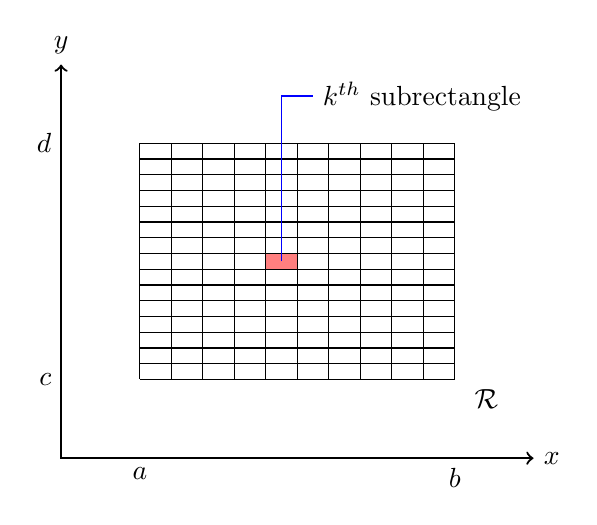
\begin{tikzpicture}[scale=2] % I should have used a \begin{axis} environment...
  \draw [<->,thick] (0,2.5) node (yaxis) [above] {$y$} |- (3,0) node (xaxis) [right] {$x$};
  \draw (0.5,0.5) -- (2.5,0.5) -- (2.5,2) -- (0.5,2) -- (0.5,0.5);
  \foreach \i in {3.5,...,11.5}{\draw (0.2*\i,0.5)  -- (0.2*\i,2);}
  \foreach \i in {6,...,19}{\draw (0.5,0.1*\i) -- (2.5,0.1*\i);}
  \draw [fill opacity=0.5,fill=red] (1.3,1.2) -- (1.3,1.3) -- (1.5,1.3) -- (1.5,1.2) -- (1.3,1.2);
  \draw [color=blue] (1.4,1.25) -- (1.4,2.3) -- (1.6,2.3);
  \node [right] at (1.6,2.3) {$k^{\text{th}}$ subrectangle};
  \node [below] at (0.5,0) {$a$};
  \node [below] at (2.5,0) {$b$};
  \node [left] at (0,0.5) {$c$};
  \node [left] at (0,2) {$d$};
  \node [below] at (2.7,0.5) {$\mathcal{R}$};
\end{tikzpicture}
\caption{$\mathcal{R}: [a,b] \times [c,d]$ partitioned.}
\end{figure}

We begin by partitioning our rectangle, which we define as $\mathcal{R}: [a,b] \times [c,d]$, into smaller subrectangles. The $x$-axis is partitioned at $x_0,x_1,\dots,x_m$ and the $y$-axis is partitioned into $y_0,y_1,\dots,y_n$. 

Within each subrectangle, we choose a point $(x_k^*,y_k^*)$ that will give us the ``best approximation'' for the volume of the prism with that subrectangle as its base. Then the volume is given by:
\[
\begin{aligned}
\text{Volume} &= \text{Area} \cdot \text{Height} \\
\text{Area} &= \Delta x_k \Delta y_k = \Delta A_k \\
\text{Height} &= f(x_k^*,y_k^*) \\
V_k &= f(x_k^*,y_k^*)\Delta A_k \\
V_{\text{solid}} &\approx \sum_{i=1}^Nf(x_k^*,y_k^*)\Delta A_k
\end{aligned}
\]
We can define $\norm{\mathcal{P}}$ to be the norm of partition (in this case, the length of the diagonal of a subrectangle. \\ \\
The \textbf{double integral} is defined by:
\[ \iint_{\mathcal{R}} f(x,y) \ dA = \lim_{\norm{\mathcal{P}} \to 0} \sum_{k=1}^N f(x_k^*,y_k^*)\Delta A_k = \lim_{m,n \to \infty} \sum_{i=1}^m\sum_{j=1}^nf(x_{ij}^*,y_{ij}^*)\Delta A_{ij} \]
This integral yields the ``signed volume'' below the surface $z = f(x,y)$, meaning that the integral can yield a negative answer.

To compute such an integral for the rectangular region $\mathcal{R}$, we perform an integral within an integral. Our expression is equivalent to:
\[ \iint_{\mathcal{R}} f(x,y) \ dA = \int_c^d\int_a^b f(x,y) \ dx \ dy \]

\subsection{Double Integrals over General Regions}
When dealing with general regions, we can divide them up into two categories:
\begin{enumerate}
\item Type I, or $x$-simple, regions, bounded by $a \le x \le b$ and $g_1(x) \le y \le g_2(x)$. In this case, our integral is \[ \int_a^b \int_{g_1(x)}^{g_2(x)}f(x,y) \ dy \ dx \]
\item Type II, or $y$-simple, regions, bounded by $c \le y \le d$ and $h_1(y) \le x \le h_2(y)$. In this case, our integral is \[ \int_c^d \int_{h_1(y)}^{h_2(y)}f(x,y) \ dx \ dy \]
\end{enumerate}

\subsection{Reversing the Order of Integration}
Because we can arbitrarily choose to integrate $x$ or $y$ first, this leads to a theorem:
\begin{theorem}[Fubini's Theorem]
If $f(x,y)$ is continuous over a rectangle $\mathcal{R}: [a,b] \times [c,d]$, then \[ \iint_{\mathcal{R}} f(x,y) \ dA = \int_c^d\int_a^b f(x,y) \ dx \ dy = \int_a^b f(x,y) \ dy \ dx \]
\end{theorem}
Fubini's Theorem only works if the bounds are constant values. If they are functions of another variable, the way to change the order of integration is by:
\begin{enumerate}
\item Sketching the region.
\item Finding the bounds on $x$ and $y$.
\item Rewriting the integral.
\end{enumerate}
We also have the following theorem:
\begin{theorem}[Separation of Variables for Iterated Integrals]
Let $g(x)$ and $h(y)$ be continuous functions on $[a,b]$ and $[c,d]$, respectively, along the $x$-axis and $y$-axis, respectively. Then $f(x,y) = g(x)h(y)$ is a continuous function in the rectangle $\mathcal{R}: [a,b] \times [c,d]$ and \[ \iint_{\mathcal{R}} f(x,y) \ dA = \int_a^bg(x) \ dx \int_c^d h(y) \ dy \]
\end{theorem}

\subsection{Triple Integrals (not covered)} % not covered
While double integrals are formed by considering small area elements in the $xy$-plane, a triple integral is formed by considering small volume elements in space. Suppose we have a box $\mathcal{B}: [a,b]\times [c,d] \times [r,s]$ in space, where $f(x,y,z)$ is defined in. We can use the same principles as in a double integral in order to create small subboxes $B_{ijk}$. Dividing $x$ into $l$ subintervals, $y$ into $m$ subintervals, and $z$ into $n$ subintervals, We omit the steps here, but it should be obvious that \[ V_{\text{box}} \approx \sum_{i=1}^l\sum_{j=1}^m\sum_{k=1}^nf(x_{ijk}^*,y_{ijk}^*,z_{ijk}^*)\Delta V_{ijk} \]
Then the triple integral is defined as: \[ \iiint_{\mathcal{B}} f(x,y,z) \ dV = \lim_{l,m,n \to \infty}\sum_{i=1}^l\sum_{j=1}^m\sum_{k=1}^nf(x_{ijk}^*,y_{ijk}^*,z_{ijk}^*)\Delta V_{ijk} \]
and calculating the integral is similar: \[ \iiint_{\mathcal{B}} f(x,y,z) \ dV = \int_r^s\int_c^d\int_a^bf(x,y,z) \ dx \ dy \ dz \]
Fubini's Theorem and the Separation of Variables Theorem still apply. \\ \\
When calculating over general solid regions, there are two types:
\begin{enumerate}
\item Type I solid regions, given by $\{(x,y,z)| (x,y) \in \mathcal{D}, u_1(x,y) \le z \le u_2(x,y) \}$ where $\mathcal{D}$ is the projection onto the $xy$ plane. In this case, our integral is \[ \iint_{\mathcal{D}}\left[\int_{u_1(x,y)}^{u_2(x,y)}f(x,y,z) \ dz\right] \ dA \]
\item Type II solid regions, given by $\{(x,y,z)| a \le x \le b, g_1(x) \le y \le g_2(x), u_1(x,y) \le z \le u_2(x,y) \}$. In this case, our integral is \[ \int_a^b\int_{g_1(x)}^{g_2(x)}\int_{u_1(x,y)}^{u_2(x,y)}f(x,y,z) \ dz \ dy \ dx \]
\end{enumerate}

\subsection{Change of Variables}
When making a change of variables within an integral, we wish to change the integral into one that is much simpler to integrate. In this case, what we are doing is changing the region we are integrating over in the $xy$-plane, and changing it into a rectangular region in some other plane, say the $uv$-plane. We do this by defining a transformation $T:(u,v) \to (x,y)$ that will allows us to transform our region into something better to work with. 

Define the \textbf{Jacobian} to be:
\[ \frac{\partial (x_1,x_2,\dots,x_n)}{\partial (u_1,u_2,\dots,u_n)} = \begin{vmatrix}
\frac{\partial x_1}{\partial u_1} & \frac{\partial x_1}{\partial u_2} & \cdots & \frac{\partial x_1}{\partial u_n} \\
\frac{\partial x_2}{\partial u_1} & \frac{\partial x_2}{\partial u_2} & \cdots & \frac{\partial x_2}{\partial u_n} \\
\vdots & \vdots & \ddots & \vdots \\
\frac{\partial x_n}{\partial u_1} & \frac{\partial x_n}{\partial u_2} & \cdots & \frac{\partial x_n}{\partial u_n}
\end{vmatrix}\]
Then we have the following result:
\begin{theorem}[Change of Variables Theorem]
Suppose $\mathcal{R}$ is a closed, bounded region in the $xy$-plane and $\mathcal{S}$ is a closed, bounded region in the $uv$-plane so that $T(u,v) = (x,y) = (g(u,v),h(u,v))$ and $T$ is one-to-one. If $f$ is continuous on $\mathcal{R}$, $g,h$ have continuous first partial derivatives, and $\frac{\partial(x,y)}{\partial (u,v)} \neq 0$ on $\mathcal{S}$, then
\[ \iint_{\mathcal{R}} f(x,y) \ dA = \iint_{\mathcal{R}}f(g(u,v),h(u,v))\left|\frac{\partial (x,y)}{\partial (u,v)}\right|  du \ dv \]
\end{theorem}

We will prove this theorem for when the region $\mathcal{R}$ is a parallelogram (we can split the region into smaller regions that we can approximate to be parallelograms). It will turn out that it is true for general regions.
\begin{proof}
\begin{figure}[h!]
\centering
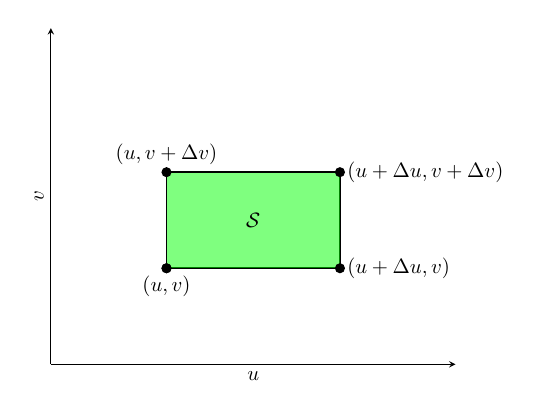
\begin{tikzpicture}[scale=0.75]
  \begin{axis} [
      axis lines=left,
      ticks=none,
      xlabel=$u$,ylabel=$v$,
      xmin=0,ymin=0,xmax=7,ymax=7,
      clip=false,
    ]
    \addplot[color=black, thick,mark color=black,mark=*] coordinates {(2,2)(5,2)(5,4)(2,4)(2,2)};
    \addplot[fill=green,fill opacity=0.5] coordinates {(2,2)(5,2)(5,4)(2,4)(2,2)};
    \node [below] at (axis cs:2,2) {$(u,v)$};
    \node [right] at (axis cs:5,2) {$(u+\Delta u,v)$};
    \node [right] at (axis cs:5,4) {$(u+\Delta u,v + \Delta v)$};
    \node [above] at (axis cs:2,4) {$(u,v+\Delta v)$};
    \node at (axis cs:3.5,3) {$\mathcal{S}$};
  \end{axis}
\end{tikzpicture}
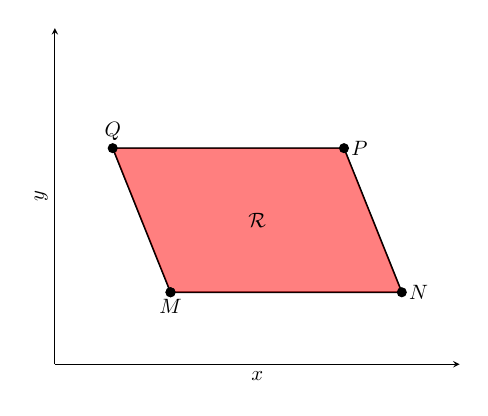
\begin{tikzpicture}[scale=0.75]
  \begin{axis} [
      axis lines=left,
      ticks=none,
      xlabel=$x$,ylabel=$y$,
      xmin=0,ymin=0,xmax=7,ymax=7,
      clip=false,
    ]
    \addplot[color=black, thick,mark color=black,mark=*] coordinates {(2,1.5)(6,1.5)(5,4.5)(1,4.5)(2,1.5)};
    \addplot[fill=red,fill opacity=0.5] coordinates {(2,1.5)(6,1.5)(5,4.5)(1,4.5)(2,1.5)};
    \node [below] at (axis cs:2,1.5) {$M$};
    \node [right] at (axis cs:6,1.5) {$N$};
    \node [right] at (axis cs:5,4.5) {$P$};
    \node [above] at (axis cs:1,4.5) {$Q$};
    \node at (axis cs:3.5,3) {$\mathcal{R}$};
  \end{axis}
\end{tikzpicture}
\end{figure}

In the above figure, let $x = g(u,v)$ and $y=h(u,v)$. Then we have the following coordinates:
\begin{itemize}
\item $M(g(u,v),h(u,v))$
\item $N(g(u+\Delta u,v),h(u+\Delta u,v))$
\item $P(g(u+\Delta u,v+\Delta v),h(u+\Delta u,v+\Delta v))$
\item $Q(g(u,v+\Delta v),h(u,v+\Delta v))$
\end{itemize}
The area of $\mathcal{S}$ is equal to $\Delta u\Delta v$. When $\Delta u, \Delta v$ are very small, \[ \text{Area of } \mathcal{R} \approx \norm{\overrightarrow{MN} \times \overrightarrow{MQ}} \]
Writing the component form of these two vectors: 
\[
\begin{aligned}
\overrightarrow{MN} &= [g(u+\Delta u,v) - g(u,v)]\ihat + [h(u+\Delta u,v) - h(u,v)]\jhat \\
\overrightarrow{MQ} &= [g(u,v+\Delta v) - g(u,v)]\ihat + [h(u,v+\Delta v) - h(u,v)]\jhat \\
\end{aligned}
\]
But also note that when $\Delta u,\Delta v$ are very small,
\[
\begin{aligned}
g_u(u,v) \approx \frac{g(u+\Delta u,v) - g(u,v)}{\Delta u} &\qquad h_u(u,v) \approx \frac{h(u+\Delta u,v) - h(u,v)}{\Delta u} \\
g_v(u,v) \approx \frac{g(u,v+\Delta v) - g(u,v)}{\Delta v} &\qquad h_v(u,v) \approx \frac{h(u,v+\Delta v) - h(u,v)}{\Delta v} \\
\end{aligned}
\]
So,
\[
\begin{aligned}
\overrightarrow{MN} &= \frac{\partial x}{\partial u}\Delta u \ihat + \frac{\partial y}{\partial u}\Delta v \jhat \\
\overrightarrow{MQ} &= \frac{\partial x}{\partial v}\Delta u \ihat + \frac{\partial y}{\partial v}\Delta v \jhat \\
\end{aligned}
\]
Therefore,
\[
\begin{aligned}
\overrightarrow{MN} \times \overrightarrow{MQ} &=
\begin{vmatrix}
\ihat & \jhat & \khat \\
\frac{\partial x}{\partial u}\Delta u & \frac{\partial y}{\partial u}\Delta u & 0 \\
\frac{\partial x}{\partial v}\Delta v & \frac{\partial y}{\partial v}\Delta v & 0 
\end{vmatrix}
= 0\ihat - 0\jhat + 
\begin{vmatrix}
\frac{\partial x}{\partial u} & \frac{\partial y}{\partial u} \\
\frac{\partial x}{\partial v} & \frac{\partial y}{\partial v} 
\end{vmatrix}
\Delta u\Delta v \khat \\
\text{Area of } \mathcal{R} &= \Delta A \approx \norm{\overrightarrow{MN} \times \overrightarrow{MQ}} \approx \left|\frac{\partial (x,y)}{\partial(u,v)}\right|du \ dv
\end{aligned}
\]
Therefore,\[ \iint_{\mathcal{R}} f(x,y) \ dA = \iint_{\mathcal{R}}f(g(u,v),h(u,v))\left|\frac{\partial (x,y)}{\partial (u,v)}\right| du \ dv \]
\end{proof}

This concept is best learned by example.\\ \\
Suppose we wish to evaluate the integral \[ \iint_{\mathcal{R}} (x+y)^2\sin^2(x-y) \ dA \] where $\mathcal{R}$ is the region bounded by the square with vertices $(0,1),(1,2),(2,1),(1,0)$. We cannot really perform this integral, so we use a change of variables. We note that the region is bounded by
\[
\begin{aligned}
1 &\le x+y \le 3 \\
-1 &\le x-y \le 1
\end{aligned}
\]
so we let $u = x+y$ and $v = x-y$. Solving for $x$ and $y$, we get $x = g(u,v) = \frac{u+v}{2}$ and $y = h(u,v) = \frac{u-v}{2}$. The Jacobian is:
\[ \frac{\partial (x,y)}{\partial (u,v)} = \begin{vmatrix}
\frac{\partial x}{\partial u} & \frac{\partial y}{\partial u} \\
\frac{\partial x}{\partial v} & \frac{\partial y}{\partial v} 
\end{vmatrix} = \begin{vmatrix}
\frac{1}{2} & \frac{1}{2} \\ \frac{1}{2} & -\frac{1}{2}
\end{vmatrix} = -\frac{1}{2} \]
So our integral becomes  \[ \iint_{\mathcal{R}} (x+y)^2\sin^2(x-y) \ dA = \int_{-1}^1\int_1^3u^2\sin^2(v) \left|-\frac{1}{2}\right| du \ dv \]
which can be computed normally (by separation of variables or by iterated integrals).
\subsection{Integrals in Special Coordinate Systems}
We omit the proofs here, but using the above technique, we can transform a Cartesian integral into the following systems:
\begin{itemize}
\item \textbf{Polar} \[ \begin{cases} x = r\cos{\theta} \\ y = r\sin{\theta} \end{cases} \] which means \[ \iint_{\mathcal{R}}f(x,y) \ dA = \iint_{\mathcal{S}}f(r\cos{\theta},r\sin{\theta}) r \ dr \ d\theta\]
\item \textbf{Cylindrical} \[ \begin{cases} x = r\cos{\theta} \\ y = r\sin{\theta} \\ z = z \end{cases} \] which means \[ \iiint_{\mathcal{B}} f(x,y,z) \ dV = \iiint_{\mathcal{G}}f(r\cos{\theta},r\sin{\theta},z) r \ dr \ d\theta \ dz \]
\item \textbf{Spherical} \[ \begin{cases} x = r\sin{\theta}\cos{\varphi} \\ y = r\sin{\theta}\sin{\varphi} \\ z = r\cos{\theta} \end{cases} \] which means \[ \iiint_{\mathcal{B}} f(x,y,z) \ dv = \iiint_{\mathcal{G}}f(r\sin{\theta}\cos{\varphi},r\sin{\theta}\sin{\varphi},r\cos{\theta}) r^2\sin{\theta} \ dr \ d\theta \ d\varphi \]
\end{itemize}
\section{Vector Calculus (not covered)} % not covered

\subsection{Line Integrals}
Line integrals deal with integrals over curves in the plane or space, in which the curve takes on certain values over a region. 

There are many forms of the line integral. First, we explore taking the line integral with respect to arc length. By partitioning a curve $\mathcal{C}$ into $n$ subintervals, we can find the value taken on by each of those subintervals with $f(x,y)$. We define the \textbf{line integral with respect to arc length} as: \[ \int_{\mathcal{C}}f(x,y) ds = \lim_{n \to \infty}\sum_{i=1}^nf(x_i^*,y_i^*)\Delta s_i \]
Recall from single-variable calculus that the arc length along a parametric curve $\mathcal{C}(t) = \la x(t), y(t) \ra$ is: \[ s(t) = \int_a^t\sqrt{\left(\frac{dx}{d\tau}\right)^2 + \left(\frac{dy}{d\tau}\right)^2} \ d\tau \]
Therefore, \[ ds = \sqrt{\left(\frac{dx}{dt}\right)^2 + \left(\frac{dy}{dt}\right)^2} \ dt \]
So another form for our line integral is:
\[ \boxed{\int_{\mathcal{C}}f(x,y) \ ds = \int_a^b f(x(t),y(t)) \sqrt{\left(\frac{dx}{dt}\right)^2 + \left(\frac{dy}{dt}\right)^2} \ dt} \]
One way to intuitively think about the line integral is as follows: if a wire follows the curve $\mathcal{C}$, and $f(x,y)$ represents the linear mass density of the wire at $(x,y)$, then the line integral will give the mass of the wire on the curve. \\ \\
We can also define line integrals with respect to $x$ and $y$ as follows:
\[
\begin{aligned}
\int_{\mathcal{C}}f(x,y) \ dx &= \int_a^b f(x(t),y(t))\frac{dx}{dt} \ dt \\
\int_{\mathcal{C}}f(x,y) \ dy &= \int_a^b f(x(t),y(t))\frac{dy}{dt} \ dt
\end{aligned}
\]

Since we usually have these two integrals appearing together, a shorthand for the sum of these two integrals is:
\[ \int_{\mathcal{C}}P(x,y) \ dx + Q(x,y) \ dy = \int_{\mathcal{C}}P(x,y) dx + \int_{\mathcal{C}} Q(x,y) dy \]

We can extend this to three dimensions easily.

Sometimes, our curve $\mathcal{C}$ may consist of multiple individual curves. In this case, the line integrals are additive, meaning we can take the integrals of each individual curve and add them. 

What happens when we take the line integral in the opposite direction? You will see that \[ \int_{-\mathcal{C}} f(x,y) \ dx + g(x,y) \ dy = -\int_{\mathcal{C}} f(x,y) \ dx + g(x,y) \ dy\] where $-\mathcal{C}$ is the curve $\mathcal{C}$ traveling in the opposite direction. 

\subsection{Work}
One of the ubiquitous applications of line integrals is the concept of work. If we have a vector field $\vec{F}(x,y)$ representing the force field at a position $(x,y)$, then it turns out the work done by the field on a particle moving along a curve $\mathcal{C}$ is \[ \int_{\mathcal{C}}\vec{F}(x,y) \cdot d\vec{r} \]
Do note that this expression merely simplifies down to our sum from above, if the curve can be described by $\vec{r}(t) = \la x(t),y(t),z(t) \ra$: \[ \int_{\mathcal{C}}\vec{F}(x,y) \cdot d\vec{r} = \int_{\mathcal{C}}F_x \ dx + F_y \ dy + F_z \ dz \]

\subsection{The Fundamental Theorem of Line Integrals}
Earlier on, we explored the concept of the gradient of a function. We can actually treat the gradient as the derivative of a function of multiple variables. This gives rise to the following theorem.
\begin{theorem}[Fundamental Theorem of Line Integrals]
Let $\mathcal{C}$ be a smooth curve given by $\vec{r}(t)$ defined from $a \le t \le b$. Let $f$ be a differentiable multivariate function with a continuous gradient vector $\grad{f}$ on $\mathcal{C}$. Then, \[ \int_{\mathcal{C}} \grad{f} \cdot d\vec{r} = f(\vec{r}(b)) - f(\vec{r}(a)) \]
\end{theorem}

\begin{proof}
\[
\begin{aligned}
\int_{\mathcal{C}} \grad{f} \cdot d\vec{r} &= \int_{\mathcal{C}} \frac{\partial f}{\partial x} dx + \frac{\partial f}{\partial y} dy \\
&= \int_a^b \left[\frac{\partial f}{\partial x}\frac{dx}{dt} + \frac{\partial f}{\partial y}\frac{dy}{dt}\right] dt \\
&= \int_a^b \frac{d}{dt}(f(x(t),y(t))) \ dt \\
&= f(x(b),y(b)) - f(x(a),y(a)) = f(\vec{r}(b)) - f(\vec{r}(a))
\end{aligned}
\]
\end{proof}

One thing to see about this theorem is that as long as we can find the ``antiderivative'' of $\grad{f}$, then it does not matter what the precise curve $\mathcal{C}$ is; any two curves with the same endpoints will give the same value of the line integral. Such a vector field $\vec{F} = \grad{f}$ is called \textbf{conservative} if it exhibits path independence. If $\vec{F}$ is the gradient of some function, then it is conservative. 

The following theorem gives a nice way to see if a vector field is conservative.
\begin{theorem}
Let $\vec{F}(x,y) = P(x,y)\ihat + Q(x,y)\jhat$ be a vector on an open simply-connected region $\mathcal{D}$; namely, a region without holes or breaks. Then \[ \frac{\partial P}{\partial y} = \frac{\partial Q}{\partial x} \] for all $(x,y) \in \mathcal{D}$, if and only if $\vec{F}$ is conservative,i.e. $\vec{F}$ is the gradient of some function.
\end{theorem}

\begin{proof}
We prove the forward direction only. By hypothesis $\vec{F}$ is the gradient of some function $\phi(x,y)$, namely, \[ \vec{F} = P\ihat + Q\jhat = \grad{\phi} = \frac{\partial \phi}{\partial x}\ihat + \frac{\partial \phi}{\partial y} \jhat\]  
Then, 
\[
\begin{aligned}
\frac{\partial P}{\partial y} &= \frac{\partial^2 \phi}{\partial y \ \partial x} \\
\frac{\partial Q}{\partial x} &= \frac{\partial^2 \phi}{\partial x \ \partial y} 
\end{aligned}
\]
By Clairaut's Theorem, $\frac{\partial P}{\partial y} = \frac{\partial Q}{\partial x}$, and the proof is complete.
\end{proof}

\subsection{Green's Theorem}
Green's Theorem relates a line integral of a simple, closed curve to a double integral of the region enclosed by the curve.

Before we state it, we define the term \textbf{positively oriented} to refer to a curve where the direction of travel for increasing $t$ is counterclockwise. 
\begin{figure}
  \centering
  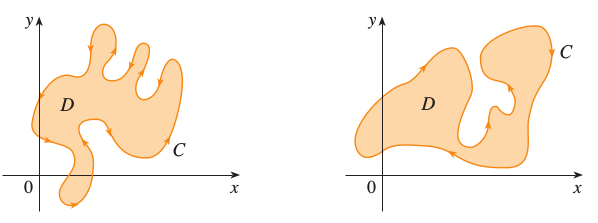
\includegraphics[scale=0.4]{curves}
  \caption{Left: Positively oriented curve. Right: Negatively oriented curve.}
\end{figure}
\begin{theorem}[Green's Theorem]
Let $\mathcal{C}$ be a positively oriented, piecewise-smooth, closed curve in the plane. Let $\mathcal{D}$ be the region bounded by $\mathcal{C}$ ($\mathcal{C}$ is denoted $\partial \mathcal{D}$). If $P(x,y)$ and $Q(x,y)$ have continuous partial derivatives on an open region containing $\mathcal{D}$, then \[ \oint_{\mathcal{C}}P \ dx + Q \ dy = \iint_{\mathcal{D}}\left(\frac{\partial Q}{\partial x} - \frac{\partial P}{\partial y}\right) \ dA \]
\end{theorem}
The loop around the integral sign means that $\mathcal{C}$ is a closed curve. 
\begin{proof}
This proof is for when $\mathcal{D}$ is both a type I and type II region. \\
\begin{center}
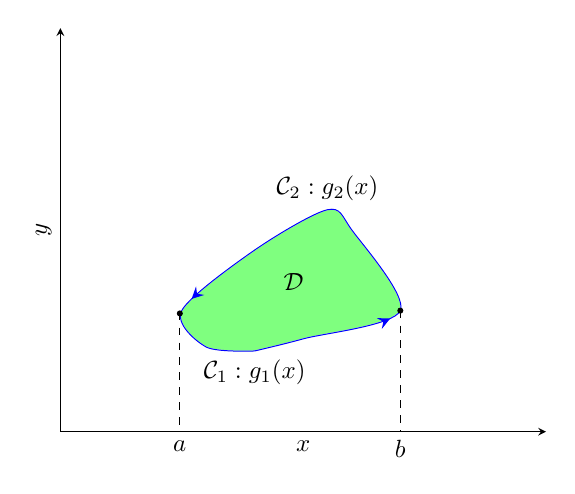
\begin{tikzpicture}[scale=0.9]
  \begin{axis}[
      axis lines=left,clip=false,ticks=none,
      xlabel=$x$,ylabel=$y$,
      xmin=0,ymin=0,xmax=10,ymax=10,
    ]
        \addplot[color=white,smooth,fill=green,fill opacity=0.5] coordinates {(4,2)(5,2.3)(7,3)(6,5)(5.5,5.5)(4,4.5)(2.5,3)(3,2.1)(4,2)};
        \addplot[blue,smooth]
        coordinates {(4,2)(5,2.3)(7,3)(6,5)(5.5,5.5)(4,4.5)(2.5,3)(3,2.1)(4,2)}
        [arrow inside={end=stealth,opt={blue,scale=1.5}}{0.25,0.8}];
        \draw[dashed] (axis cs:2.46,2.95) -- (axis cs:2.46,0);
        \draw[dashed] (axis cs:7,3) -- (axis cs:7,0);
        \draw [fill=black] (axis cs:2.46,2.93) circle (1pt);
        \draw [fill=black] (axis cs:7,3) circle (1pt);        
        \node[below] at (axis cs:2.46,0) {$a$};
        \node[below] at (axis cs:7,0) {$b$};
        \node[below] at (axis cs:4,2) {$\mathcal{C}_1: g_1(x)$};
        \node[above] at (axis cs:5.5,5.5) {$\mathcal{C}_2: g_2(x)$};
        \node at (axis cs:4.8,3.7) {$\mathcal{D}$};
  \end{axis}
\end{tikzpicture}
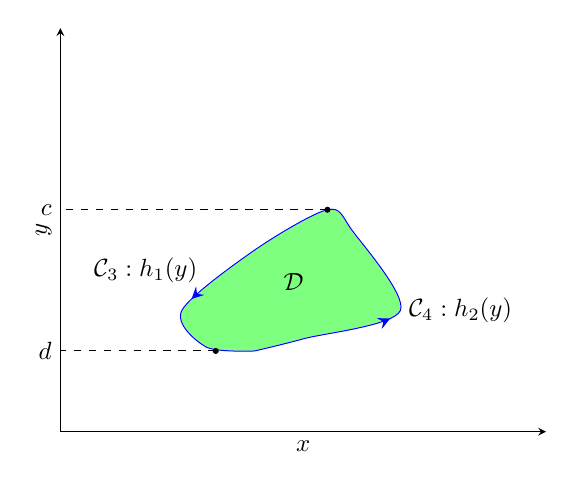
\begin{tikzpicture}[scale=0.9]
  \begin{axis}[
      axis lines=left,clip=false,ticks=none,
      xlabel=$x$,ylabel=$y$,
      xmin=0,ymin=0,xmax=10,ymax=10,
    ]
    \addplot[color=white,smooth,fill=green,fill opacity=0.5] coordinates {(4,2)(5,2.3)(7,3)(6,5)(5.5,5.5)(4,4.5)(2.5,3)(3,2.1)(4,2)};
        \addplot[blue,smooth]
        coordinates {(4,2)(5,2.3)(7,3)(6,5)(5.5,5.5)(4,4.5)(2.5,3)(3,2.1)(4,2)}
        [arrow inside={end=stealth,opt={blue,scale=1.5}}{0.25,0.8}];
        \draw[dashed] (axis cs:5.5,5.5) -- (axis cs:0,5.5);
        \draw[dashed] (axis cs:3.2,2) -- (axis cs:0,2);
        \draw [fill=black] (axis cs:5.5,5.5) circle (1pt);
        \draw [fill=black] (axis cs:3.2,2) circle (1pt);        
        \node[left] at (axis cs:0,5.5) {$c$};
        \node[left] at (axis cs:0,2) {$d$};
        \node[left] at (axis cs:3,4) {$\mathcal{C}_3:h_1(y)$};
        \node[right] at (axis cs:7,3) {$\mathcal{C}_4:h_2(y)$};
        \node at (axis cs:4.8,3.7) {$\mathcal{D}$};
  \end{axis}
\end{tikzpicture}
\end{center}
We wish to prove the following:
\[ \int_{\mathcal{C}}P(x,y) \ dx = - \iint_{\mathcal{D}} \frac{\partial P}{\partial y} \ dA \qquad \text{and} \qquad \int_{\mathcal{C}}Q(x,y) \ dx = \iint_{\mathcal{D}}\frac{\partial Q}{\partial x} \ dA \]
To prove the first condition, treat $\mathcal{D}$ as type I. Then, since $\mathcal{C} = \mathcal{C}_1 \cup \mathcal{C}_2$, \[ \int_{\mathcal{C}}P(x,y) \ dx = \int_{\mathcal{C}_1}P(x,y) \ dx + \int_{\mathcal{C}_2}P(x,y) \ dx \]
To simplify our calculations, we write \[ \oint_{\mathcal{C}}P(x,y) \ dx = \int_{\mathcal{C}_1}P(x,y) \ dx - \int_{-\mathcal{C}_2}P(x,y) \ dx \]
since now we can describe our curves $\mathcal{C}_1$ and $\mathcal{C}_2$ as:
\[
\begin{aligned}
C_1&: x = t, y = g_1(t) \qquad (a \le t \le b) \\
-C_2&: x = t, y = g_2(t) \qquad (a \le t \le b) \\
\end{aligned}
\]
Then,
\[
\begin{aligned}
\int_{\mathcal{C}}P(x,y) \ dx &= \int_a^bPf(t,g_1(t)) \left(\frac{dx}{dt}\right) \ dt - \int_a^b P(t,g_2(t))\left(\frac{dx}{dt}\right) \ dt \\
&= \int_a^b P(t,g_1(t)) \ dt - \int_a^b P(t,g_2(t)) \ dt \\
&= -\int_a^b P(t,y)\biggl|_{y=g_1(t)}^{y=g_2(t)} \ dt \\
&= -\int_a^b \int_{g_1(t)}^{g_2(t)}\frac{\partial P}{\partial y} \ dy \ dt = -\int_a^b \int_{g_1(x)}^{g_2(x)}\frac{\partial P}{\partial y} \ dy \ dt \\
&= -\iint_{\mathcal{D}}\frac{\partial P}{\partial y} \ dA
\end{aligned}
\]
Using a similar argument by treating $\mathcal{D}$ as a type II region, we ultimately get \[ \int_{\mathcal{C}}Q(x,y) \ dy = \iint_{\mathcal{D}}\frac{\partial Q}{\partial x} \ dA \]
Adding these two gives the statement of the theorem, and we're done. 
\end{proof}

We can use Green's Theorem to find the area enclosed by a closed curve. Since the area of a region is given by \[ \iint_{\mathcal{D}}dA \] we need \[ \frac{\partial Q}{\partial x} - \frac{\partial P}{\partial y} = 1 \]
We can choose different things for $P$ and $Q$:
\begin{itemize}
\item $P(x,y) = -y$, $Q(x,y) = 0$ 
\item $P(x,y) = 0$, $Q(x,y) = x$
\item $P(x,y) = -\frac{1}{2}y$, $Q(x,y) = \frac{1}{2}x$
\end{itemize}
Therefore,
\[ \boxed{A = -\oint_{\mathcal{C}}y \ dx = \oint_{\mathcal{C}}x \ dy = \frac{1}{2}\oint_{\mathcal{C}}-y \ dx + x \ dy} \]

\subsection{Green's Theorem for General Regions}
If we can divide a region up into multiple simple regions, we can apply Green's Theorem to those simple regions and add the values up to obtain a cumulative value. \\ \\
We can also apply it to when a region has a hole.
\begin{center}
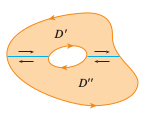
\includegraphics[scale=0.4]{holes}
\end{center}
If the outside curve is $\mathcal{C}_1$ and the inside is $\mathcal{C}_2$, we apply Green's Theorem to get \[ \begin{aligned} \iint_{\mathcal{D}}\left(\frac{\partial Q}{\partial x} - \frac{\partial P}{\partial y}\right) \ dA &= \iint_{\mathcal{D}'}\left(\frac{\partial Q}{\partial x} - \frac{\partial P}{\partial y}\right) \ dA + \iint_{\mathcal{D}''}\left(\frac{\partial Q}{\partial x} - \frac{\partial P}{\partial y}\right) \ dA \\ &= \int_{\partial \mathcal{D}'}P \ dx + Q \ dy + \int_{\partial \mathcal{D}''}P \ dx + Q \ dy \end{aligned} \]
The boundaries shared between $\mathcal{D}'$ and $\mathcal{D}''$ cancel each other out, so we remain at \[  \iint_{\mathcal{D}}\left(\frac{\partial Q}{\partial x} - \frac{\partial P}{\partial y}\right) \ dA = \int_{\mathcal{C}_1}P \ dx + Q \ dy + \int_{\mathcal{C}_2}P \ dx + Q \ dy = \int_{\mathcal{C}}P \ dx + Q \ dy \]
and thus Green's Theorem stands.
\subsection{Parametric Surfaces}
A parametric surface is of the form \[ \vec{r}(u,v) = x(u,v)\ihat + y(u,v)\jhat + z(u,v)\khat \]
\subsection{Surface Integrals}


\subsection{Divergence Theorem}

\subsection{Stokes' Theorem}

\end{document}
